\chapter{The Level 1 trigger upgrade} % 
\label{cha:triggerUpgrade}

During Run 2, the LHC has provided collisions at an energy of 13\TeV~and at  
a peak luminosity of $14\times10^{33}cm^{-2}s^{-1}$, marking a signifcant increase
in peak energy and luminosity provided during Run 1 (8\TeV~and $7\times10^{33}cm^{-2}s^{-1}$).
With a spacing between bunches of 25ns an average of 25 simlutaneous interactions are 
produced per bunch crossing. This high luminosity and pileup provides a challenging
environment for the L1 trigger system during Run 2, which must continue to provide 
an input rate to the HLT of 100kHz, in conditions that exceed design specifications. 
Simply increasing thresholds on the L1 trigger seeds would cause
unacceptable inefficiencies for electroweak physics and \TeV~scale searches
and, therefore, the L1 trigger system, and associated algorithms, must be upgraded. 

In this section, the upgrades to the L1 calorimetric trigger system and the 
associated L1 jet algorithm are discussed. The muon trigger system 
and upgrades to the algorithms for identification of other physics objects for 
the L1 trigger are detailed in~\cite{ele_algo,tau_algo,muon_algo}.


\section{Legacy system and upgrade}

The Global Calorimeter Trigger (GCT) was used during Run 1 to find jets, electrons and photons and to 
compute global energy sums \cite{gct}. The trigger system takes input from trigger towers (TTs) 
corresponding to $5\times5$ ECAL crystals and an identical area in the HCAL. 
These are grouped into $4\times4$ \emph{calorimeter regions} which formed the input for physics object and
reconstruction algorithms for the GCT. Trigger Primitive Generators (TPGs) provide the interface
with the detector to compute trigger inputs. Due to hardware limitations the detector is split into 16 
sections each processed by a Regional Calorimetric Trigger (RCT) to form candidates and sum 
energies. The RCTs must share information to account for features which occur at boundaries between 
the 16 sections. The information from the RCTs is combined in the GCT which computes global quantities and sorts 
the jets before passing these quantities to the Global Trigger (GT). The GT also receives information 
from the Global Muon Trigger (GMT) and makes the final trigger decision. 

The upgrade of the GCT was carried out in two stages. The first stage,
Upgrade Calorimetric Trigger (UCT), was used for data taking during 2015
and used updated firmware and algorithms to allow improved jet and object 
identification, including pileup subtraction \cite{uct}. In the second stage the 
architecture was entirely replaced by the Time Multiplexed Trigger (TMT) 
to allow \emph{time multiplexing}, whereby each
event is processed entirely within one card using the full trigger tower granularity. 

\section{The Time Multiplexed Trigger architecture}

The TMT uses two processing layers. The first, \emph{layer one}, performs
pre-processing and data formatting using 18 CTP7 cards \cite{mp7}. Each card requires
only a regional view of the detector and performs local operations such as summing 
ECAL and HCAL transverse energies. The data for each event is combined and transmitted to 
a single node in the second processing layer, an Imperial Master Processor Virtex-7 (MP7) card \cite{mp7}. 
The MP7 is a high performance 0.92Tb/s + 0.92Tb/s (input + output rate) all-optical processor 
with sufficient data rate for the entire calorimeter to be processed in a single card. The data 
from the 9 nodes on layer two is passed to a demultiplexer board (also an MP7) before
being sent to the GT. The GT makes the final trigger decision using both the calorimeter
and muon trigger systems.

The difference between the GCT/UCT and TMT architectures is shown schematically in Figure~\ref{tmux}. 
In the TMT architecture, data is buffered and retransmitted to the first node (on layer 2)
over 9 bunch crossings to allow the entire event to be processed on one card. This
removes the need for a large number of links between cards and allows the full trigger
tower granularity to be used. The increase in granularity compared to the GCT is
illustrated in Figure~\ref{fig:inputres}. 

\begin{figure}

\centering
    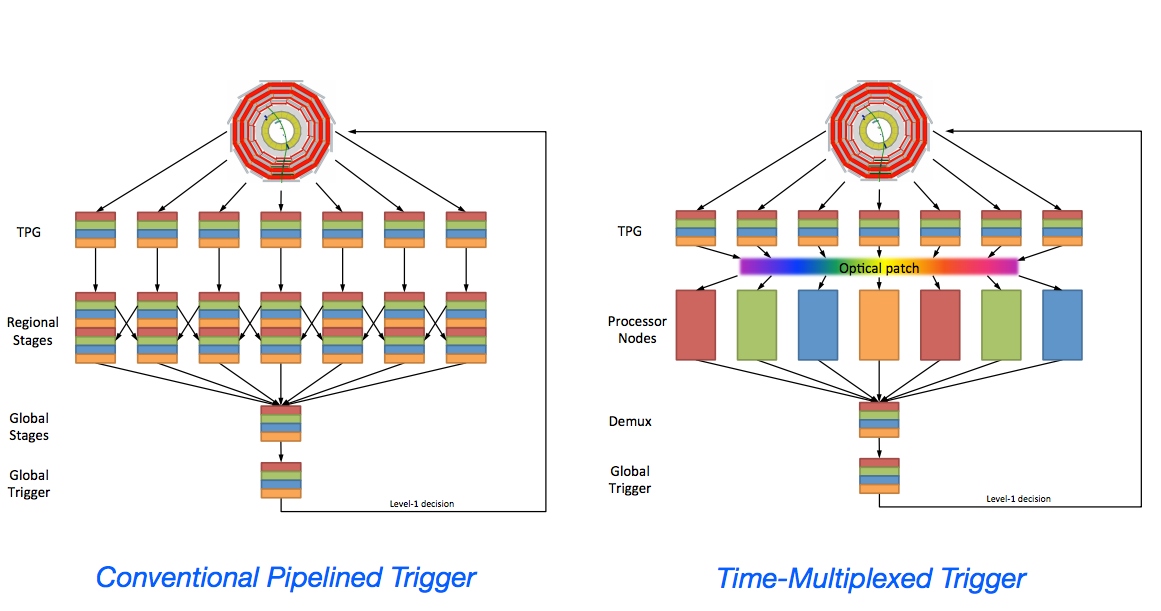
\includegraphics[width=0.9\textwidth]{./Figures/triggerUpgrade/tmux}
  \caption{Comparison of the GCT (left) and TMT architectures (right) showing the flow of information
  to the final global decision. The colours indicate the data from each bunch crossing. \cite{tmt}}
  \label{tmux}
\end{figure}

\begin{figure}
\centering
\subfigure[Input resolution: GCT]{
\includegraphics[width=0.5\textwidth]{./Figures/triggerUpgrade/L1inputreslegacy.png}\label{subfig:inputlegacy}} \quad
\subfigure[Input resolution: TMT]{
\includegraphics[width=0.5\textwidth]{./Figures/triggerUpgrade/L1inputresupgrade.png}\label{subfig:inputupgrade}} 
\caption{A representation of the CMS collaboration logo digitised with the input resolution of the L1 calorimeter trigger up to 
\etaabs~$< 3$ using (a) the legacy system ($18 \times 14$ pixels) and (b) the TMT ($72 \times 56$ pixels).}
\label{fig:inputres}
\end{figure}

\section{L1 jet algorithm}
\label{algo}

The increase in pileup and luminosity in Run 2 makes triggering with jets
significantly more challenging than during Run 1. To maintain sensitivity to
new physics the upgrade jet identification and reconstruction 
algorithm must provide high efficiencies and low rates for L1 trigger seeds.
This performance must be maintained for high pileup scenarios.

The TMT architecture provides several advantages over the GCT system which can be 
exploited in designing the jet algorithm. These include significantly increased processing power
and granularity (enhanced by factor 16). More flexible algorithms, which 
exploit smaller features than previously accessible, can be defined. This is exploited in the 
use of an improved jet clustering algorithm, described in Section~\ref{sec:jet_algo}, as well as 
online pileup subtraction, described in Section~\ref{sec:pileup_algo}, for jet 
identification and reconstruction with the TMT.

\subsection{L1 jet clustering}
\label{sec:jet_algo}
The GCT algorithm uses a $3\times3$ calorimeter region sliding jet window with a central seed 
to reconstruction jets in the range $|\eta| < 5$. The algorithm scans the calorimeter in increments
of calorimeter regions and clusters a jet if the energy in the central seed region is greater than 
both $5\GeV$ and each of the eight bordering regions. The threshold of $5\GeV$ was added during 
the 2012 8\TeV run, when the number of pileup interactions increased, to remove soft pileup jets.
The $12\times12$ TT jet size ($\Delta\eta\times\Delta\phi = 1.04\times1.04$) corresponds 
approximately to $R=0.5$ for the anti$k_T$ jet algorithm used in offline reconstruction.

The jet algorithm used for the TMT similarly uses a sliding window algorithm. This
is composed of $9\times9$ TTs ($\Delta\eta\times\Delta\phi = 0.78\times0.78$), corresponding 
to the $R=0.4$ used in Run 2. The use of an odd number of trigger towers ensures a central 
seed tower can be defined. 

In order to ensure that jets do not overlap, which would cause energy deposits 
to be double counted, the seed tower is required to meet the conditions
shown in Figure~\ref{mask}. The veto conditions are asymmetric along the diagonal to prevent  
TTs with the same energy vetoing one another. An inefficiency may be expected 
if a jet vetoes another which itself vetoes a third. However, this effect was found to 
introduce a negligible (~0.1\%) inefficiency. A threshold on the central seed tower may 
additionally be required to reconstruct a jet, as discussed in Section~\ref{sec:seed_thresh}. 

If a seed passes the veto requirements a jet is defined with a position 
given by the seed tower and an energy given by the total energy of the towers
making up the jet. The seed position is used as jets tend to be boosted
 objects with an energy deposited in a small central area. 
Note that the L1 jets are massless such that $\pt = \Et$.

\begin{figure}
\centering
    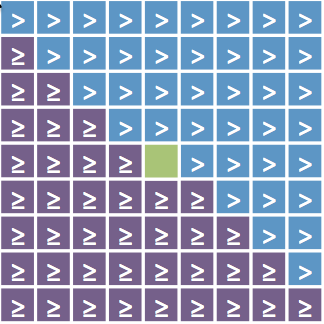
\includegraphics[width=0.5\textwidth]{./Figures/triggerUpgrade/mask.png}
  \caption{The $9\times9$ veto conditions used to define jets. The inequalities ensure
  jet energies are not double counted}
  \label{mask}
\end{figure}

\subsection{Comparison with offline jet reconstruction}

An evaluation of the performance of the L1 jet algorithm can be made by comparing
the results of jet finding with the offline reconstruction algorithm used by 
most CMS analyses during Run 2, anti-$k_T$ with a distance
parameter of 0.4, described in Section~\ref{sec:jet_reco}. 

The trigger tower deposits were generated using a simulated sample of 
top pair-production (\ttj) \footnote{In this section all simulated samples used have conditions 
of $\sqrt(s) = 13TeV$, bunch spacing $50ns$ and pileup Gaussian distributed around $40$ simultaneous interactions.} 
due to the plentiful sample of jets produced in this process. The anti-$k_T$ algorithm is run over the same inputs as
used for the L1 algorithm with the \FASTJET package~\cite{fastjet}.

A comparison between the predictions of both algorithms is shown for several important jet variables in 
Figure~\ref{fig:jet_l1s2_compak4} for the leading and fourth jet. In general, excellent agreement is observed. 
Small differences can be seen at high $|\eta|$ and low\pt. This is due to the ability 
of the anti$k_T$ algorithm to reconstruct smaller jets with smaller radii while the L1 jet
algorithm size is fixed.


\begin{figure}
\centering
    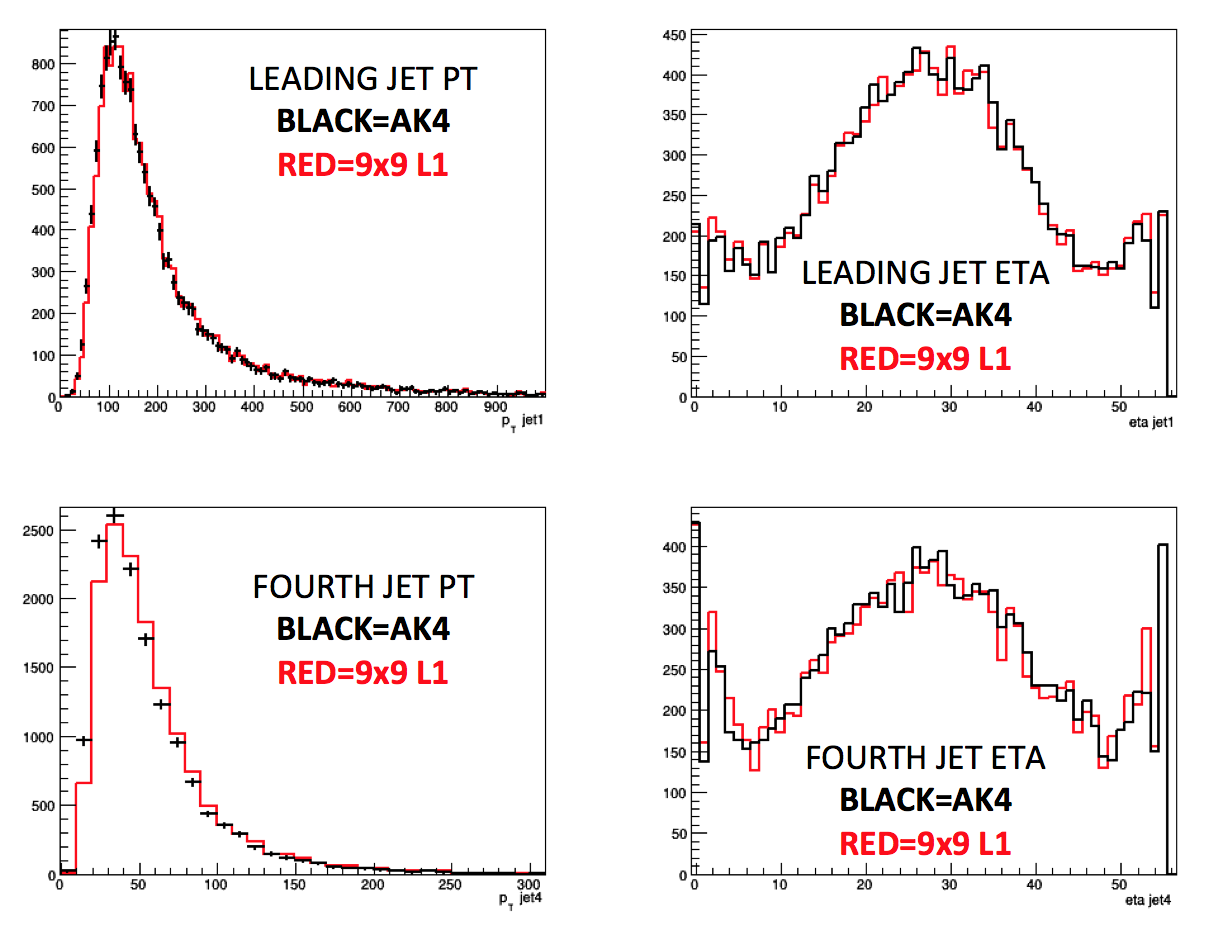
\includegraphics[width=0.8\textwidth]{./Figures/triggerUpgrade/jet_l1s2_compak4}
  \caption{Comparison of the L1 jet finding algorithm with the anti-$k_T$ algorithm using
  trigger tower inputs. Distributions of \pt~and $\eta$ are shown for the leading and fourth
  jet.}
  \label{fig:jet_l1s2_compak4}
\end{figure}  
\subsection{Energy sums}

In addition to jet reconstruction, the TMT must also build energy sums. 
These can be defined using either jets or individual calorimeter deposits, analogously to
the offline quantities. The baseline quantities that are constructed are

\begin{itemize}
\item L1 total \Et -- the scalar sum the $E_T$ of all calorimeter TTs;
\item L1 \met -- the inverse vector sum of the $E_T$ of all calorimeter TTs;
\item L1 \scalht -- the scalar sum of all L1 jet~\pt;
\item L1 \mht -- the inverse vector sum of all L1 jet~\pt.
\end{itemize}

The quantities made using L1 jets require a minimum \pt of 20\GeV. As will be discussed in 
Section~\ref{sec:trig_perf}, this requirement provides additional robustness against soft
jet reconstructed from detector noise or pileup. Additional quantities based 
on jets and/or energy sums may also be used to define trigger seeds. 
A study of the performance of one such variable is detailed in Section~\ref{sec:cross_trigger}.

\section{Pileup subtraction}
\label{sec:pileup_algo}
Simultaneous soft interactions cause additional energy to be deposited throughout
the detector. This will be approximately isotropically distributed ($\sim1\GeV$ per unit area), however, variations
in detector response as well as the profile of pileup events can cause $\eta$ and,
to a lesser extent $\phi$ dependence. In addition, event-by-event fluctuations in the distribution 
and magnitude of the pileup deposits can greatly affect calorimeter objects. 
For jets, pileup can both increase the energy of jets associated to the hard 
scatter as well as causing \emph{pileup jets} to be clustered 
entirely from pileup energy deposits.

Pileup subtraction at L1 aims to remove pileup contributions such that the trigger
decision is unbiased by the presence of simultaneous interactions. Changes during running
to detector response and beam conditions as well as the random nature of pileup necessitate an event-by-event
estimation and mitigation of the pileup contribution. For the TMT, this must be done using only the calorimeter as 
tracker information is unavailable. 

Several methods of pileup subtraction that meet the stringent latency requirement
are discussed in this section. These rely on both global and local estimations of 
pileup in each event to perform pileup correction and reject pileup jets. 
Local methods are more susceptible to statistical fluctuations, however,
unlike global methods, they allow anisotropy in the 
pileup distribution to be considered.

\subsection{Global $\rho$~subtraction}

Global $\rho$~subtraction uses the jets themselves to estimate the pileup energy density~(\rhoP) using
the median energy density of all jets in the event, defined as \rhoG~\cite{jet_area}. 
The main assumptions in this method are that the pileup distribution is independent of $\eta$ and $\phi$,  
and the number of pileup jets is much larger than the number from the hard scatter. Using \rhoG, 
a correction to each jet can be made

\begin{equation}
\label{equ:global_rho}
p_{Tj}^{\text{subtracted}} = p_{Tj}^{\text{raw}} - \rho_{\text{global}} \cdot A_j,
\end{equation}


where $A_j$ is the area of the jet, $\Delta\phi\Delta\eta(\eta)$ (the $eta$ dependence in the area is due 
to variation in the jet tower size). If $\rho \cdot A_j > p_{Tj}^{\text{raw}}$ the jet is discarded. 
Figure~\ref{fig:medianNint} shows a strong linear dependence between \rhoG~and the number of interactions for
minimum bias events. The non-zero intercept is caused by contamination of jets from the hard scatter.

To account for $\eta$ dependence in the pileup, the \rhoG~subtraction may be amended by
dividing the calorimeter into strips of phi and calculating the median $\rho$ for jets in each 
strip. However, this local $\rho$ significantly adds to the latency in the pileup subtraction and may 
be less robust as fewer jets can be sampled in each $\eta$ slice. This \emph{local $\rho$} 
is therefore not considered in this section.

\begin{figure}
\centering
    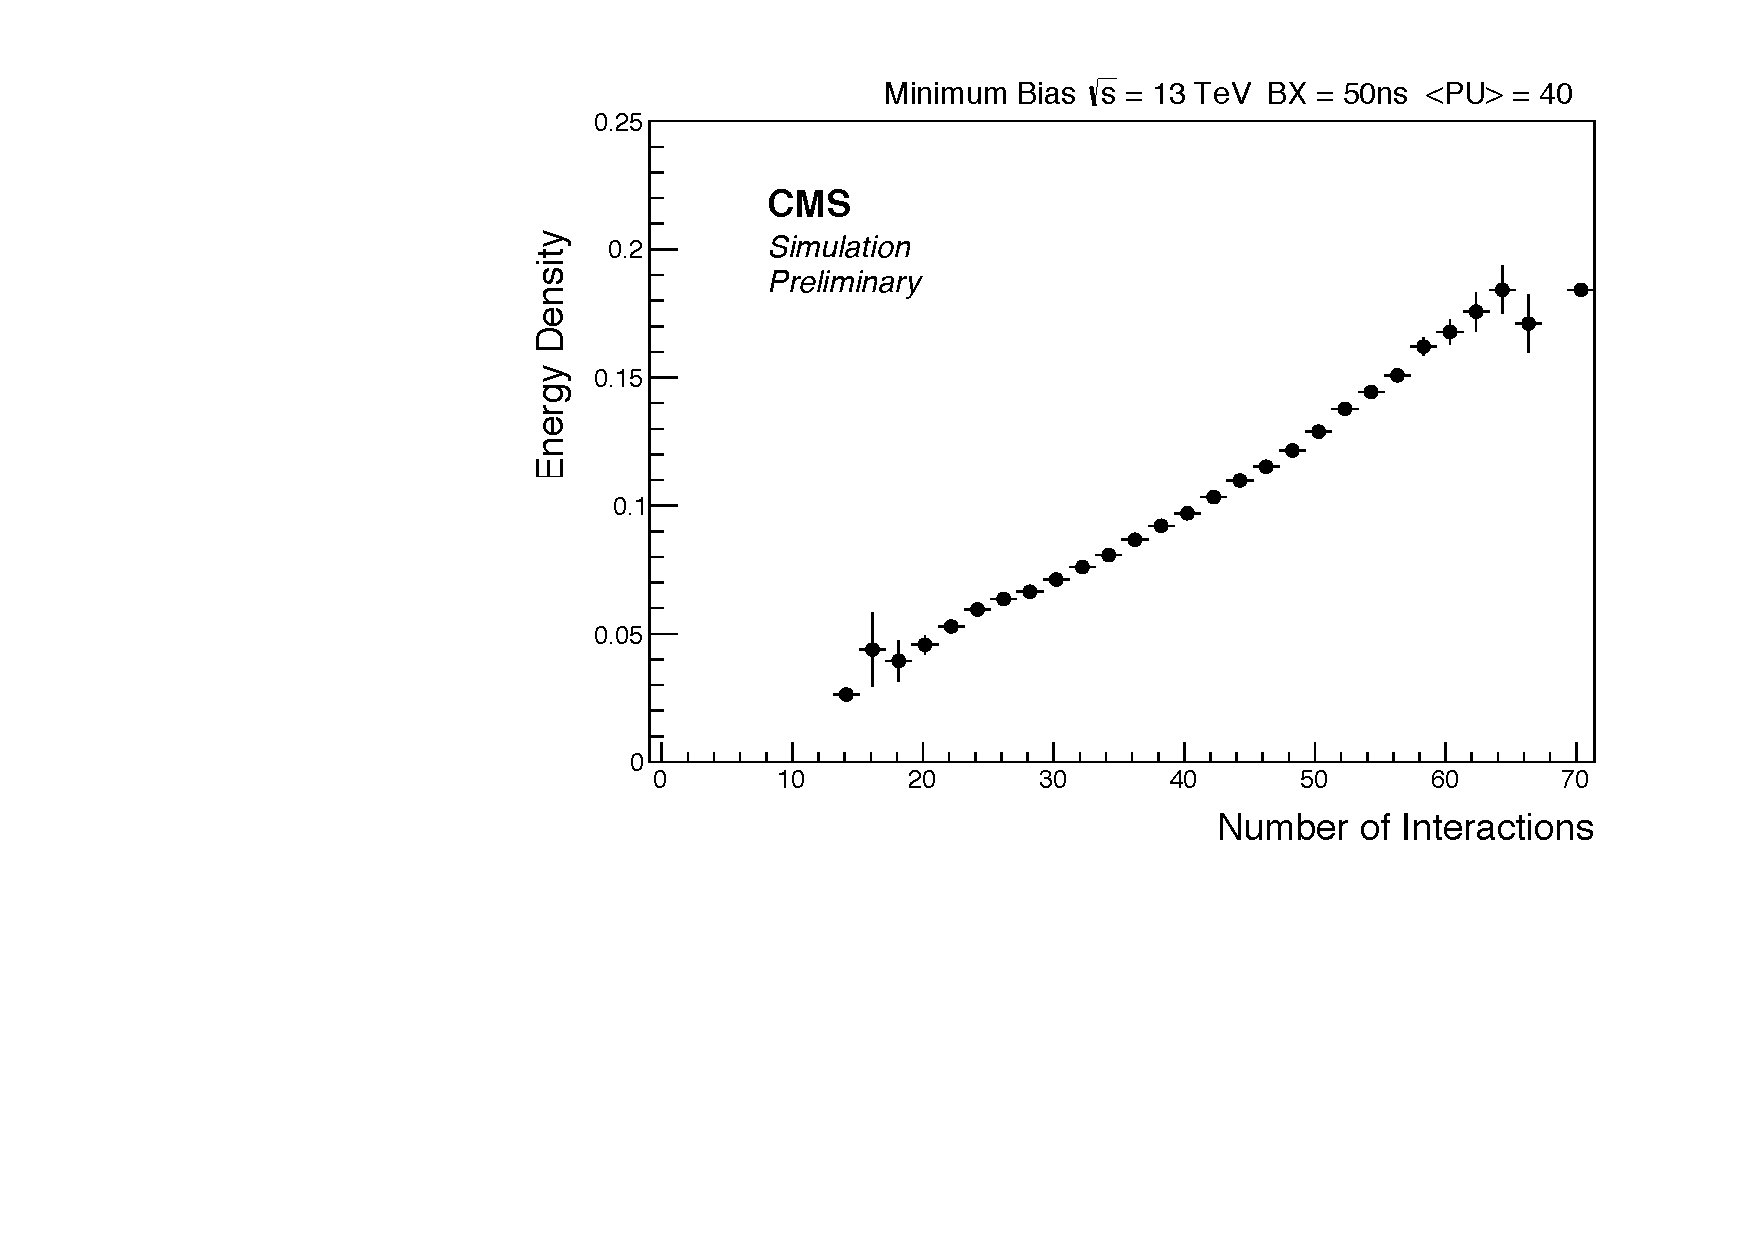
\includegraphics[width=0.8\textwidth]{./Figures/triggerUpgrade/median}
  \caption{Dependence of \rhoG (arbitrary units) on the number of interactions}
  \label{fig:medianNint}
\end{figure}  

\subsection{Doughnut subtraction}
\begin{figure}
\centering
    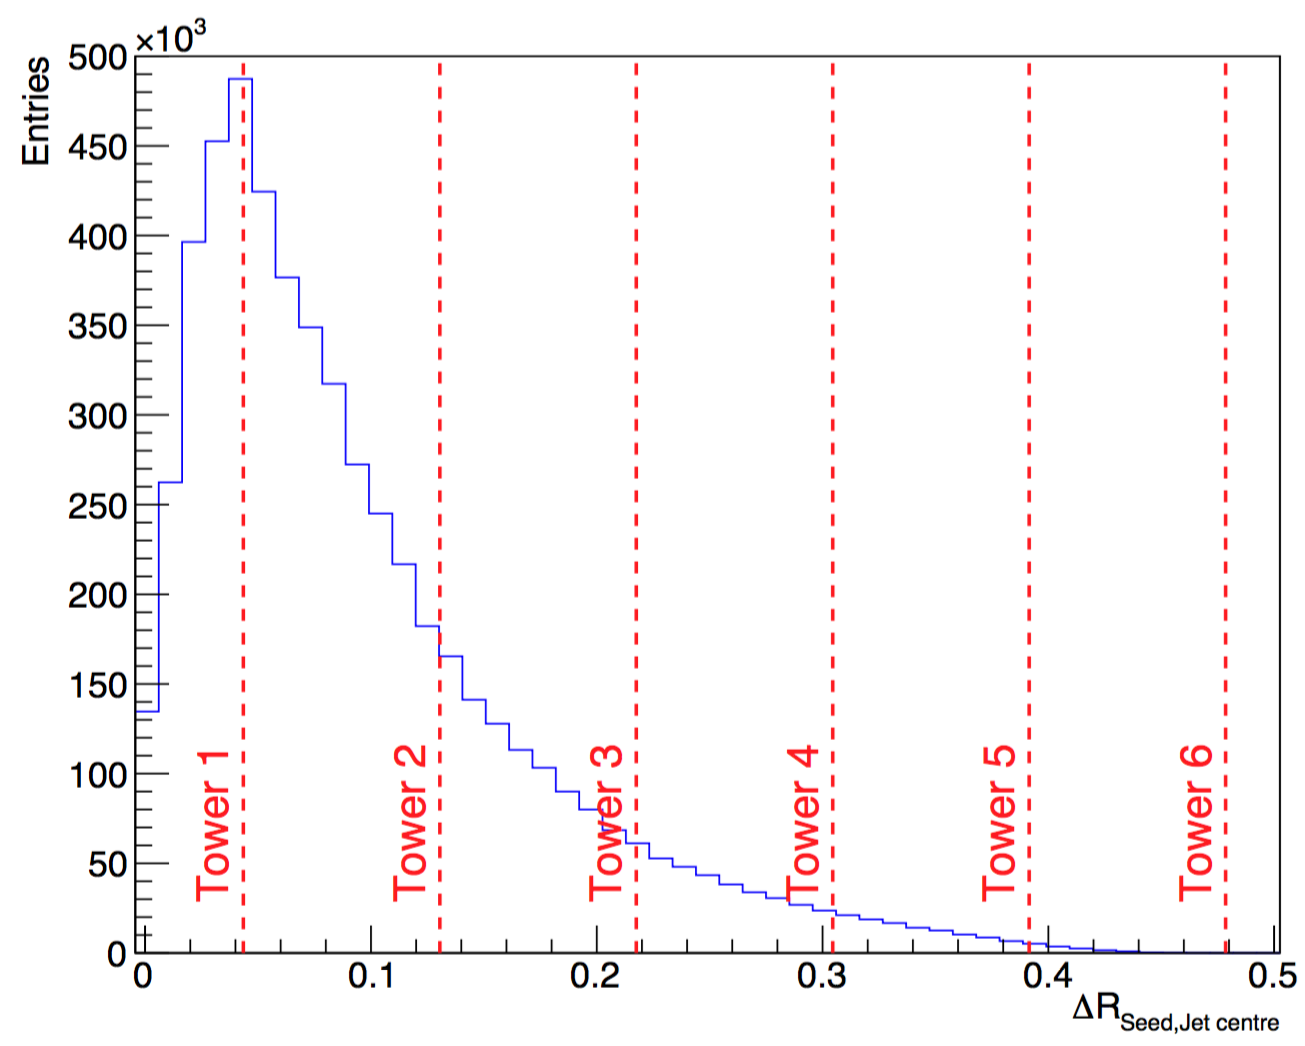
\includegraphics[width=0.8\textwidth]{./Figures/triggerUpgrade/deltaR2}
  \caption{$\Delta R$ distribution between the seed and constituent TTs using data from Run 1~\cite{mark-thesis}.}
  \label{fig:deltaR2}
\end{figure}  


Doughnut subtraction makes use of the area around the jet to sample the local pile-up
energy density in order to correct (or reject) each jet and has been previously proposed
for use during heavy ion collisions~\cite{doughnut}. The energy contribution from the jet
itself is negligible outside the $9\times9$ ring as shown in Figure~\ref{fig:deltaR2}. 
For doughnut subtraction the transverse energy density is sampled by taking four strips around 
the jet as shown in Figure~\ref{fig:donut}. The strips are ordered according to energy density,
and the median two strips taken. The pileup energy density estimated from the 
energy density of the median two strips. This \rhoD~is used to correct the
jet analogously to Equation~\ref{equ:global_rho}. Typically the strip with the largest
energy density is susceptible to contribution from nearby jets. Using the median 
strips to estimate \rhoP~allows such contamination to be mitigated.

Unlike global subtraction, doughnut subtraction allows local variations in \rhoP~to be 
included, however, it is significantly more susceptible to statistical fluctuations due to the 
reasonably small area sampled. An extension, \emph{chunky} doughnut, shown in Figure~\ref{fig:chunkyDonut},
uses enlarged strips to sample three times the area in measuring~$\rhoP$. The dependence of the number of interactions
with the energy density for the chunky doughnut pileup estimation (\rhoC) is shown in Figure~\ref{fig:threestripNint}.

\begin{figure}
\hfill
\subfigure[Doughnut rings\label{fig:donut}]{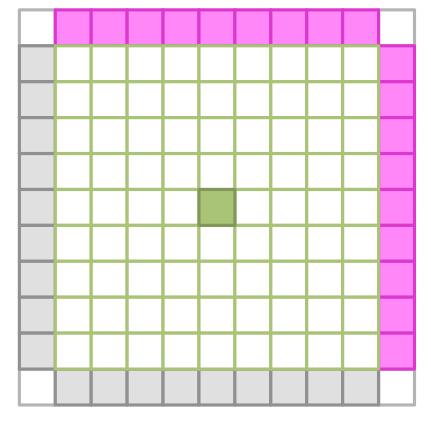
\includegraphics[width=7cm]{./Figures/triggerUpgrade/donut}}
\hfill
\subfigure[Chunky doughnut rings\label{fig:chunkyDonut}]{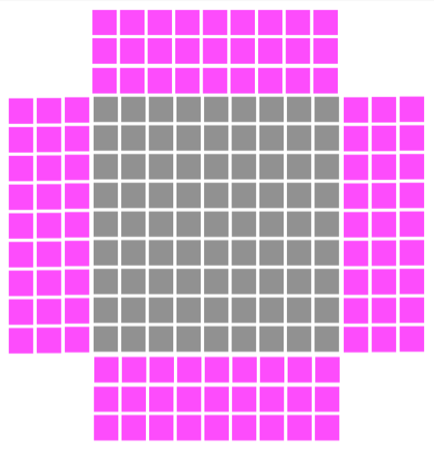
\includegraphics[width=7cm]{./Figures/triggerUpgrade/chunkyDonut}}
\hfill
\caption{The rings used to sample the local pileup energy density for the doughnut (a) and chunky doughnut (b)
pileup subtraction. The median two strips (in energy density) are used in each case.}
\end{figure}

\begin{figure}
\centering
    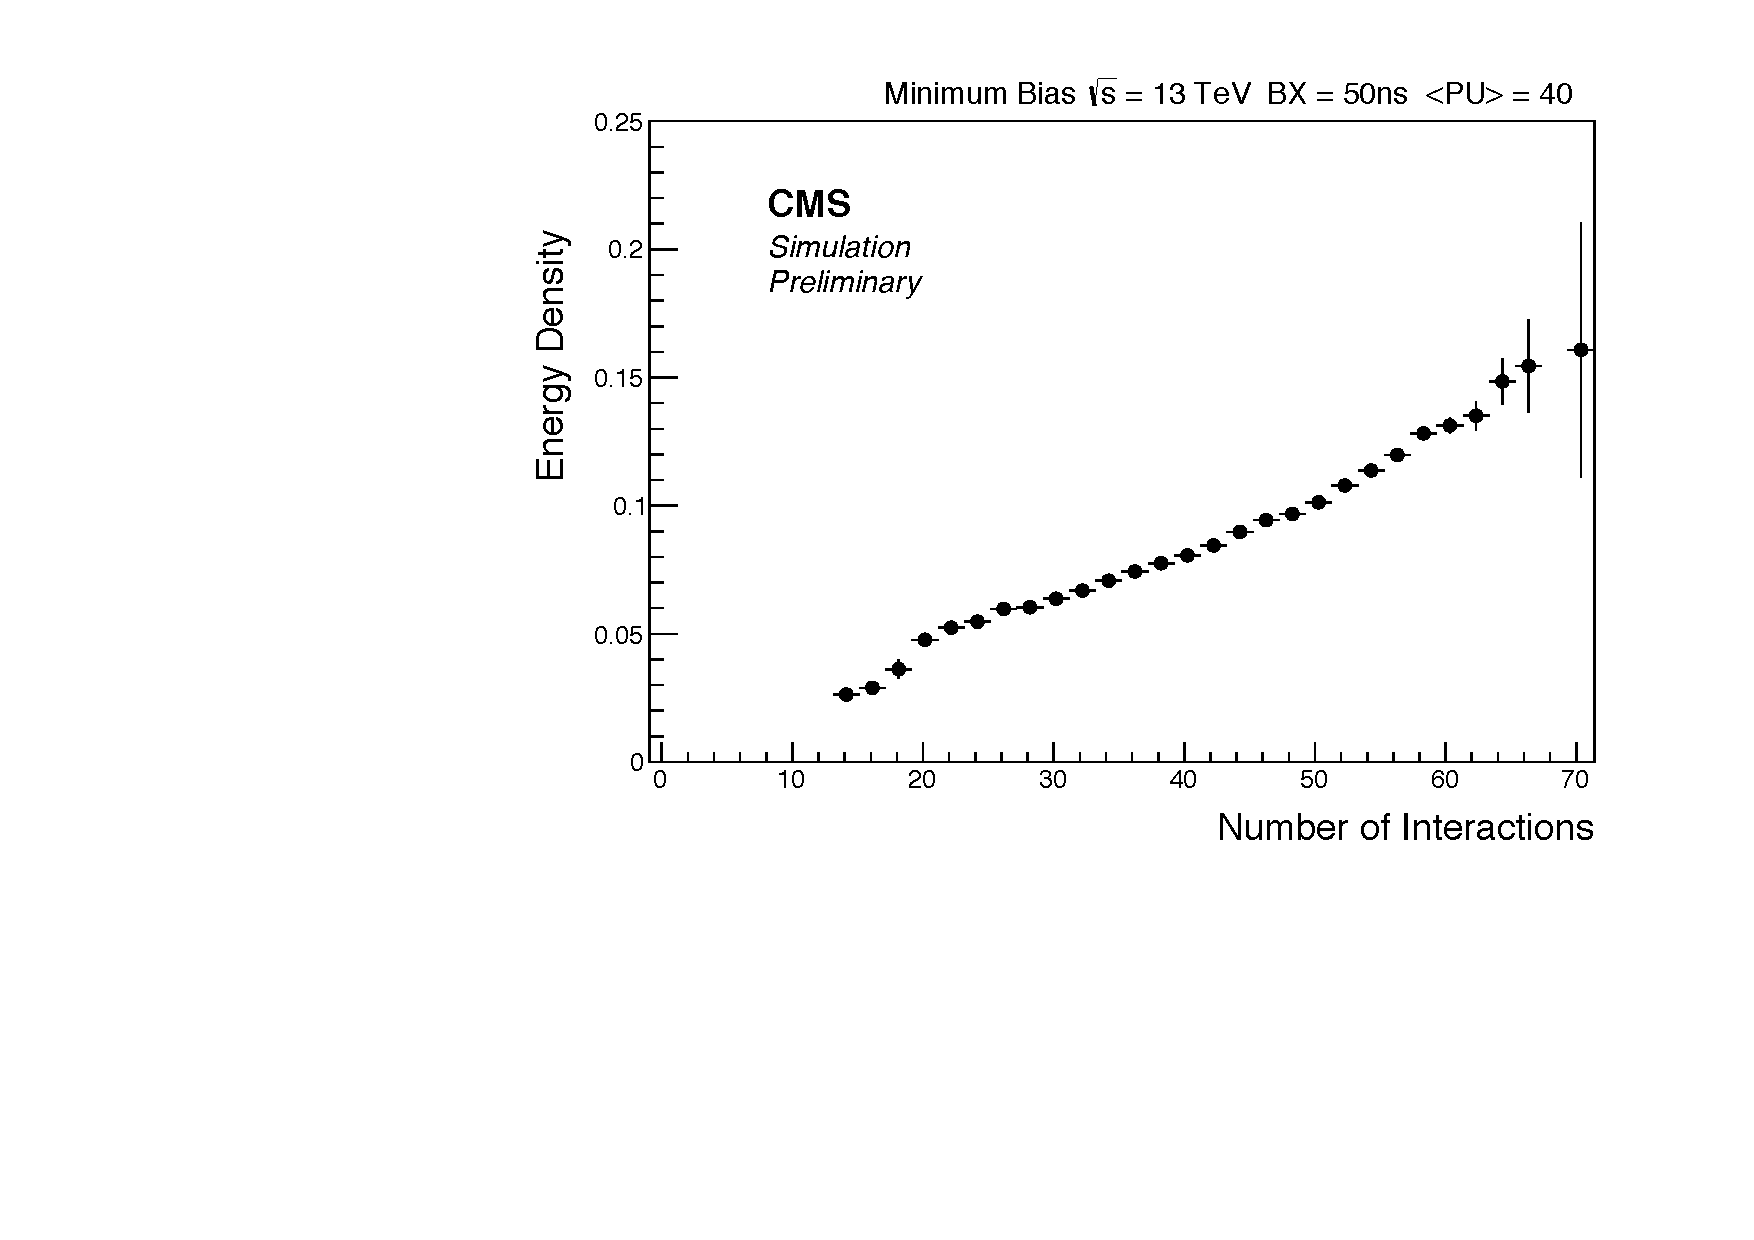
\includegraphics[width=0.8\textwidth]{./Figures/triggerUpgrade/threestrips}
  \caption{Dependence of \rhoC~(arbitrary units) on the number of interactions}
  \label{fig:threestripNint}
\end{figure}  

\subsection{Seed threshold and zero suppression}
\label{sec:seed_thresh}

The requirement of a threshold on the seed tower when identifying a jet
provides a powerful rejection of pileup jets. This takes advantage of the
diffuser energy deposition for pileup jets compared to jets originating from 
the hard scatter. A seed threshold does not allow pileup contamination in real jets to be corrected
but can be used in conjunction with other pileup subtraction techniques such as doughnut
subtraction. Global~$\rho$ subtraction is incompatible with a seed threshold as this technique relies
on reconstructing substantially more pileup jets than those from the hard scatter. 
This problem may be addressed by using a separate jet collection with no seed threshold
for calculating $\rhoG$, however, latency constraints do not permit this for the L1 trigger.

Zero suppression is a rudimentary form of pileup correction whereby only towers with
an energy deposition above a given threshold are included in the reconstruction of each jet.
This cannot be easily adapted for different pileup regimes but provides a simple baseline 
for assessing more complex algorithms. Zero suppression may also be used in conjunction
with other pileup correction techniques. 

The thresholds used for the seed and zero suppression may be $\eta$ (or even $\phi$) dependant, however,
such variable thresholds are not considered in the studies presented below. The smallest energy quanta
available at L1 is 0.5\GeV and defines a \emph{L1 unit}. The thresholds considered in this section are 5 L1 units
for the central seed (seed 5) and 1 or 2 L1 units for the zero suppression (TSup1 or TSup2).

\subsection{Calibration}
\label{sec:calib}
The energy of the L1 jets (\Lonept) is calibrated against generator level quantities using a simulated QCD dijet sample 
The calibration is carried out separately in the eight $\Delta\eta = 0.75$ ranges from $\eta=-3.0\rightarrow3.0$ 
to account for changes in detector response. In each region the procedure is as follows

\begin{itemize}
\item Cluster generator particles in the QCD sample (except muons and neutrinos) using the anti-$k_T$ algorithm with R = 0.4 into \emph{generator} jets
\item Match L1 jets to generator jets by finding the closest in $\Delta R$ between the central tower of the L1 jet and the generator jet. L1 jets with 
$\Delta R > 0.3$ from any generator jet are ignored.
\item Define the \emph{response} for each L1 jet as the ratio of the (pileup corrected) \Lonept~to the matched generator jet $pt$ (\Genpt).
\item For each bin in \Genpt, fit the response with a Gaussian to obtain the mean response for that \Genpt. 
The average \Lonept~in the bin is calculated to obtain the distribution of the mean response against \Lonept.
\item Perform a $\chi^2$ fit of the distribution of mean response against \Lonept~using the calibration
 function~\cite{l1jet_calibration}~defined in Equation~\ref{equ:jecfit}.
\item Use the result of the fit to define correction factors for each \Lonept~in each $\eta$ bin.
\end{itemize}

\begin{equation}
\left<\Lonept/\Genpt\right>^{-1} = \Lonept \cdot \left ( p_{0} + 
\frac{p_{1}}{(\log \Lonept)^{2}+p_{2}}+p_{3} \exp(-p_{4}
(\log \Lonept-p_{5} ) ^{2}) \right )
\label{equ:jecfit}
\end{equation}

The calibration must be done separately for each choice of pileup subtraction algorithm, seed threshold and zero suppression. 
An example response for \emph{seed 5}, chunky doughnut corrected jets is shown as a function of \Lonept~for 
the $0. < \eta < 0.75$ range in Figure~\ref{response}. The fitted calibration function defines the correction 
factors and is shown to agree well with the data.

In Figure~\ref{fig:closure_response} the response for the same QCD dijet sample is shown as a function of the \Lonept. The calibration
is effective for $\Lonept > \sim 20\GeV$ where the response is flat at unity. Below this \pt,
the matching procedure degrades (the majority of matched jets come from pileup or detector noise) 
such that the average response is an unreliable estimate of the jet algorithm response to real jets.

\begin{figure}
\centering
    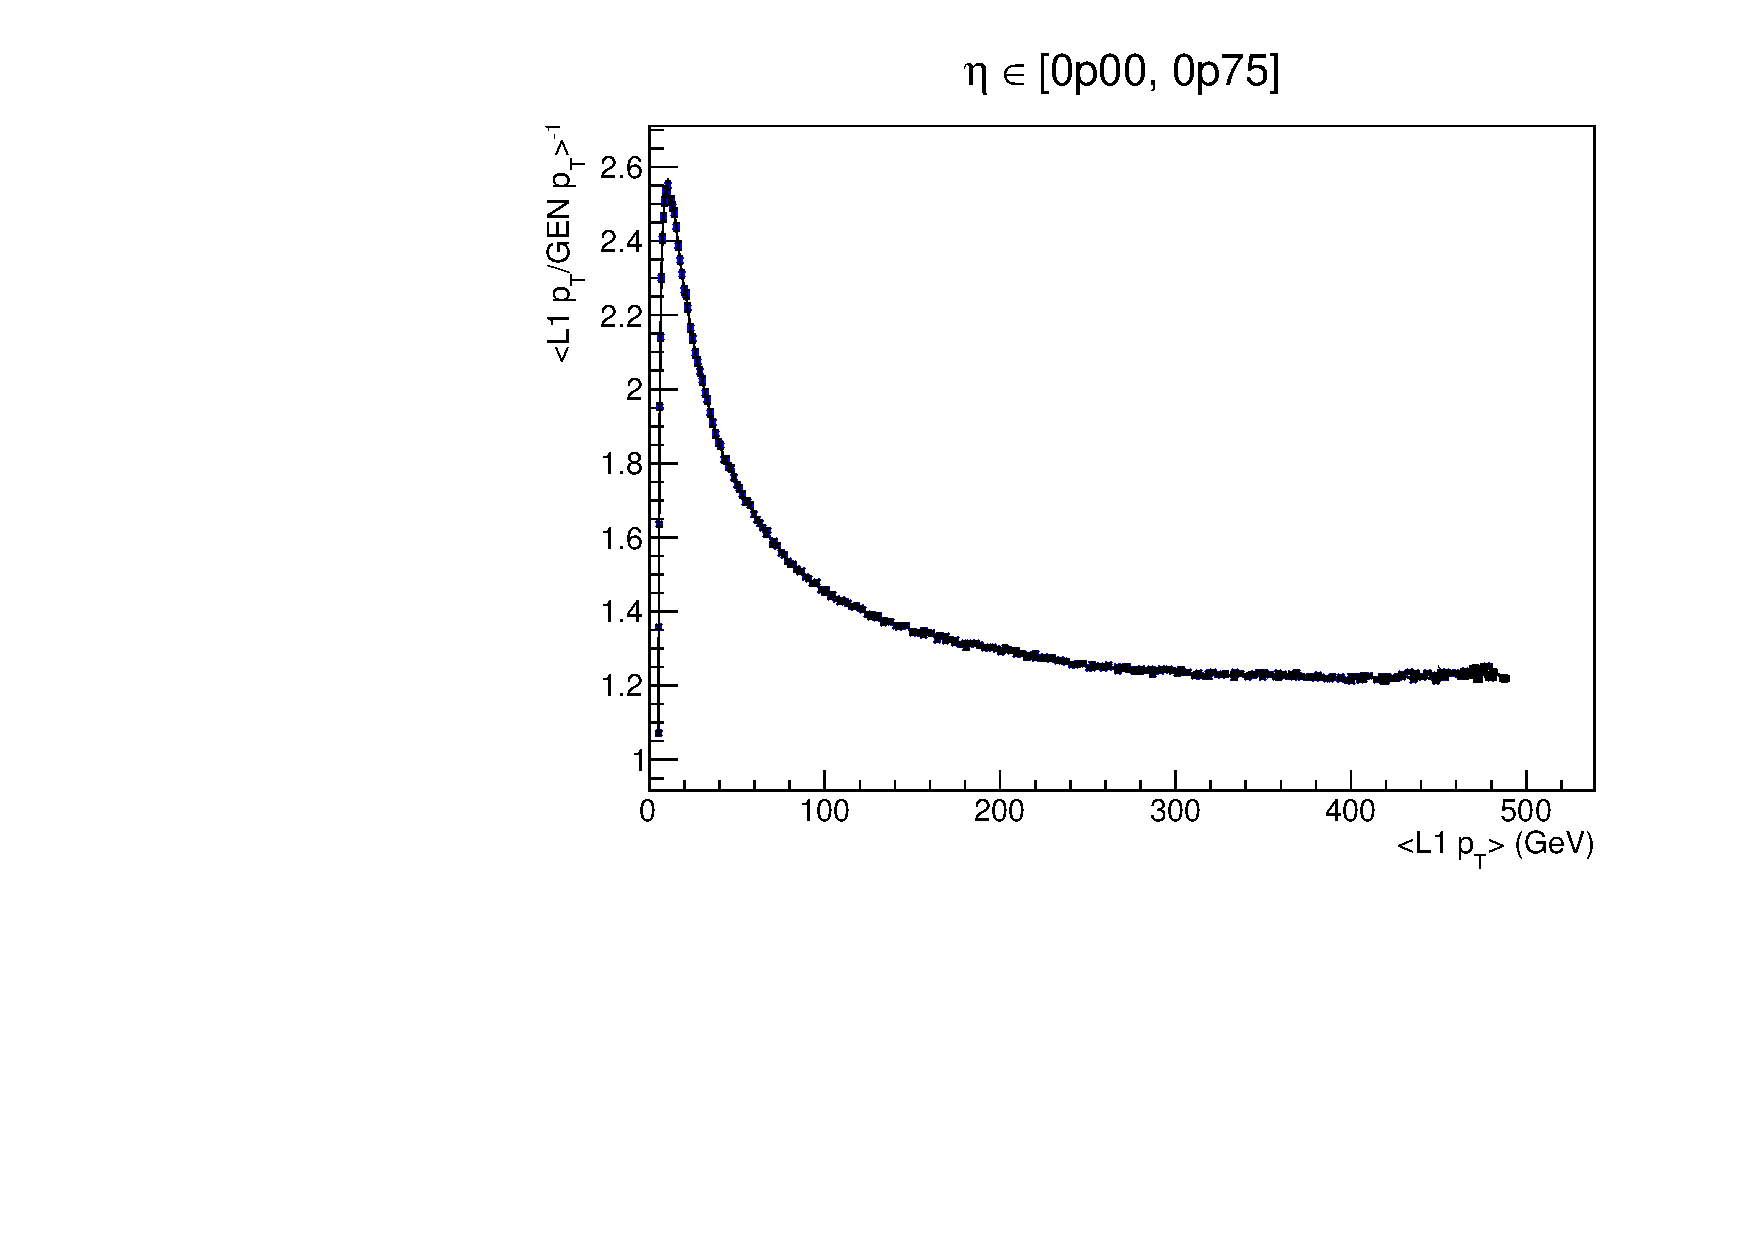
\includegraphics[width=0.8\textwidth]{./Figures/triggerUpgrade/calibrationSeed5Chunky}
  \caption{
  Fitted response for a QCD dijet sample in the range $0. < \eta < 0.75$ }
  \label{fig:response}
\end{figure}

\begin{figure}
\centering
    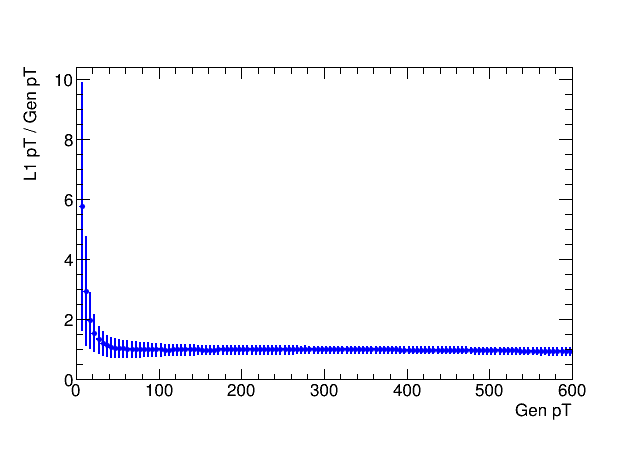
\includegraphics[width=0.8\textwidth]{./Figures/triggerUpgrade/calib_s5_chunky}
  \caption{Calibrated response in the QCD dijet sample used to derive the calibration factors. The calibration is seen to be 
  effective for the range $\Lonept > \sim 20\GeV$.}
  \label{fig:closure_response}
\end{figure}

\section{Jet performance}
\label{sec:trig_perf}
The performance of the jet algorithm and the various pileup suppression techniques is tested using
Monte Carlo simulation. In each case, the corrected \Lonept~is calibrated following the procedure in Section~\ref{sec:calib}.
Comparisons are made with algorithms used for both the legacy GCT and UCT systems to benchmark the performance.
Efficiencies are measured using a simulated \ttbar sample while 
background rates are measured using a simulated minimum bias sample.

\subsection{Matching efficiency}

The matching efficiency to generator jets provides a measure of the ability of the L1 jet algorithm 
to reconstruct real jets from the hard scatter. The matching procedure is the same as that used for the calibration. 
The matching efficiency for all generator jets and the fourth leading jet is shown 
in Figure~\ref{fig:match} as a function of $\Genpt$ for several benchmark pileup suppression algorithms. 
The efficiency plateaus at unity around $\Genpt=50\GeV$. The pileup subtraction and seed threshold is shown to reduce
the matching efficiency at low $p_T$, however, for this low $p_T$ region the L1 jets matched to generator jets are typically
reconstructed from pileup calorimeter deposits and their energy does not therefore
reflect that of the matched generator jet. A substantial improvement in efficiency over the GCT is observed in 
matching the fourth leading jet.


% The matching efficiency does not fully describe the performance as L1 jets matched to generated jets may be reconstructed
% from pileup energy deposits. The resolution is observed to plateau at unity for $\Genpt > \sim30\GeV$.


%%WOULD LIKE PLOT HERE!!

\begin{figure}
\begin{center}
\subfigure[All jets\label{fig:label:alljet}]{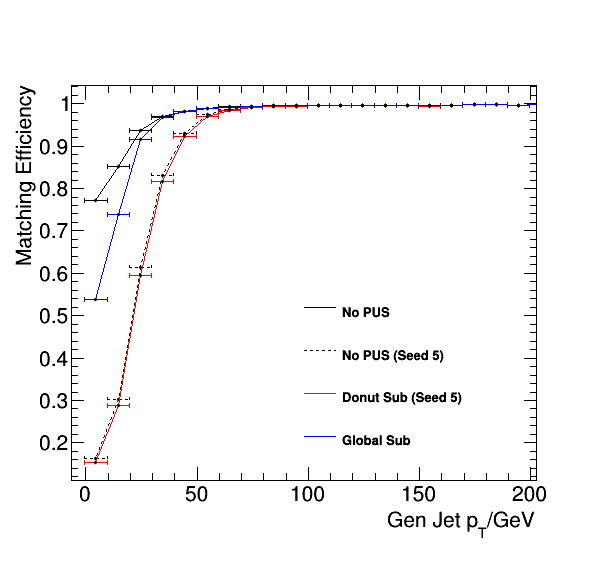
\includegraphics[width=0.5\textwidth]{./Figures/triggerUpgrade/alljet}}
\subfigure[4th jet\label{fig:label:jet4}]{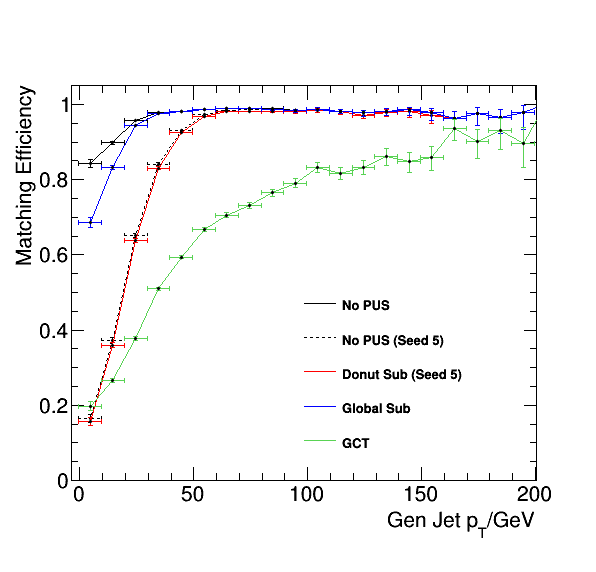
\includegraphics[width=0.5\textwidth]{./Figures/triggerUpgrade/jet4}}
\caption{Matching efficiencies for jets showing effect of seed and pileup subtraction at low energies. In \ref{fig:label:jet4} 
a comparison with the GCT is shown.}
\label{match}
\end{center}
\end{figure}

\subsection{Resolution}

The resolution, defined as $(\Lonept-\Genpt)/\Genpt$, measures the level of agreement between the energies of the 
L1 and matched generator jets. The matching procedure is the same as that described in \Section~{sec:calib}.
The resolution provides an important measure of the ability of the algorithm to reject jets from pileup
energy deposits as well as to remove the contribution of pileup from real jets from the hard scatter.
In Figure~\ref{fig:resolution1}, the resolution as a function of the number of simultaneous interactions is shown for
a simulated \ttbar sample. The resolution is flat near unity when pileup subtraction is applied,
but exhibits a strong dependence on pileup if uncorrected. To illustrate the pileup contamination for different
\Genpt~jets, a linear fit to the resolution as a function of pileup is made in \Genpt~bins and the resultant gradients
shown in Figure~\ref{fig:resolution2}. Pileup subtraction is shown to significantly reduce the 
pileup dependence of the resolution across $\Genpt$. If no pileup subtraction is applied, 
the magnitude of the gradient is particularly enhanced for low \Genpt~where pileup contamination dominates. 

\begin{figure}
    \begin{center} 
	\subfigure[\label{fig:resolution1}]{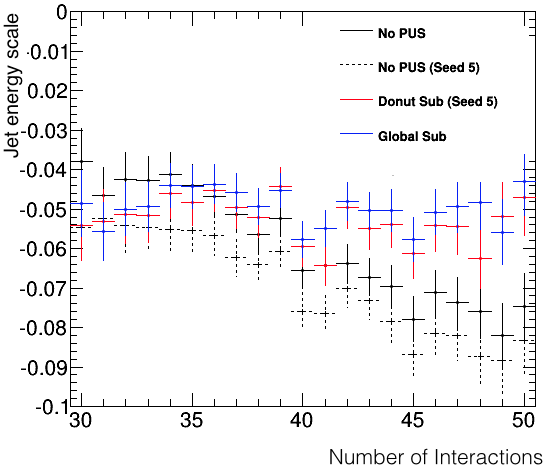
\includegraphics[width=0.5\textwidth]{./Figures/triggerUpgrade/resolution}}~
	\subfigure[\label{fig:resolution2}]{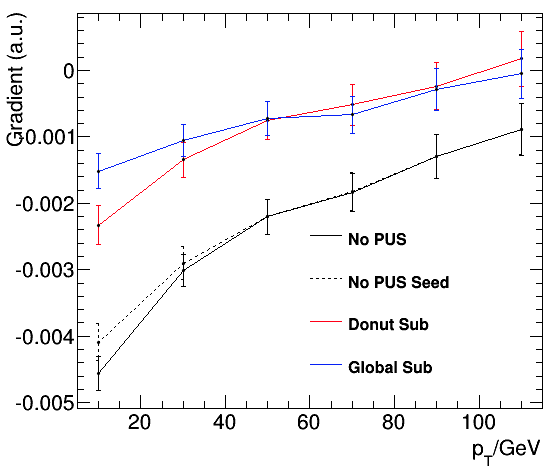
\includegraphics[width=0.5\textwidth]{./Figures/triggerUpgrade/p1eta_14to28_calib_fits}}
	\caption{(a) Resolution as a function of the number of interactions. (b) Gradients of linear fits to 
	    resolution as a function of number of interactions in bins of $p^{gen}_{T}$.}
	    \label{fig:label:resolution}
    \end{center} 
\end{figure}

\subsection{Rates and efficiencies}

The \emph{turn on} of the efficiency for generator quantities for a L1 selection of 150\GeV~on the leading jet
and 100\GeV~on the fourth leading jet are shown in Figure \ref{fig:turnon}. The upgrade trigger exhibits a sharper turn on
than the GCT quantities and plateaus at higher values than the legacy system. 

\begin{figure}
    \begin{center} 
	\subfigure[\label{fig:resolution1}]{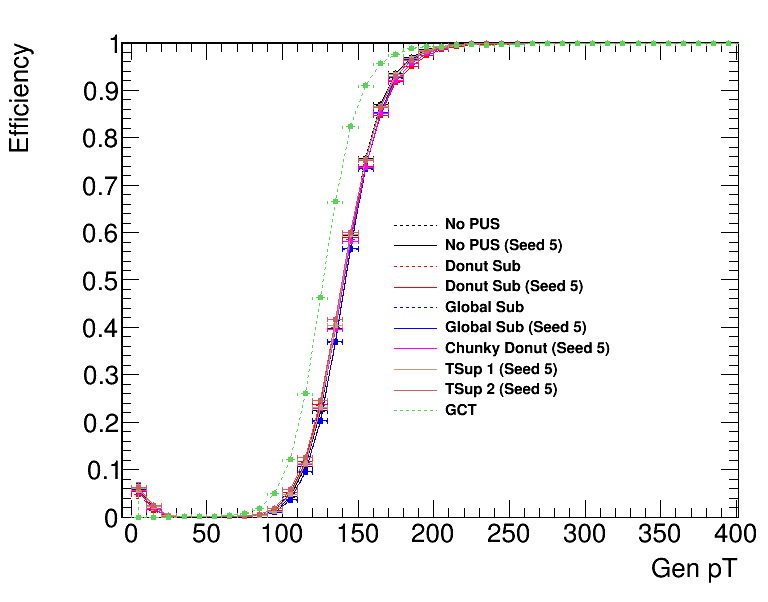
\includegraphics[width=0.5\textwidth]{./Figures/triggerUpgrade/leadJet150_noUct}}~
	\subfigure[\label{fig:resolution2}]{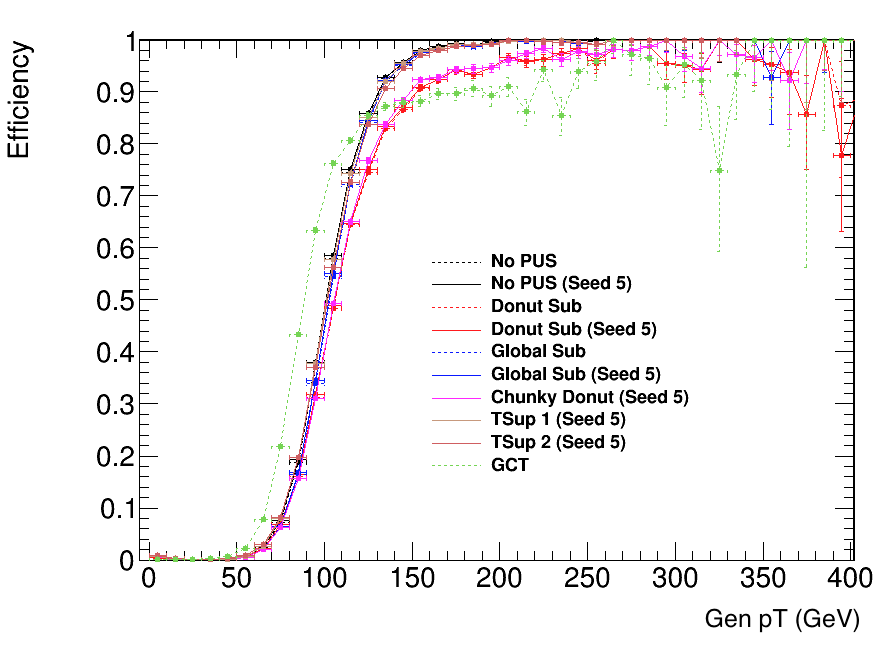
\includegraphics[width=0.5\textwidth]{./Figures/triggerUpgrade/fourthJet100_noUct}}
	\caption{Efficiency as a function of $\Genpt$ for (a) a L1 threshold of 150\GeV~on the leading jet and (b) 
	a L1 threshold of 100\GeV~on the fourth leading jet.}
	    \label{fig:turnon}
    \end{center} 
\end{figure}

The efficiencies shown in Figure~\ref{fig:turnon}, however, do not fully describe the performance 
of the trigger as the total rate of selected events must be considered as this places 
stringent restrictions on the possible L1 thresholds. Figure~\ref{fig:rate_eff_jets} shows the rate of 
minimum bias events passing selection (per second) against the efficiencies for selecting 
a leading jet, second leading jet and fourth leading jet with $\Genpt$ thresholds of $150\GeV$,
$100\GeV$ and $50\GeV$ respectively. As the jet multiplicity increases and threshold decreases
the performance of the upgrade L1 jets compared to the legacy system is substantially improved.
For the upgrade L1 jets, the global $\rho$~subtraction exhibits the best performance, however, the differences 
between the pileup subtraction algorithms are small.

\begin{figure}[h!]
  \centering
    \subfigure[]{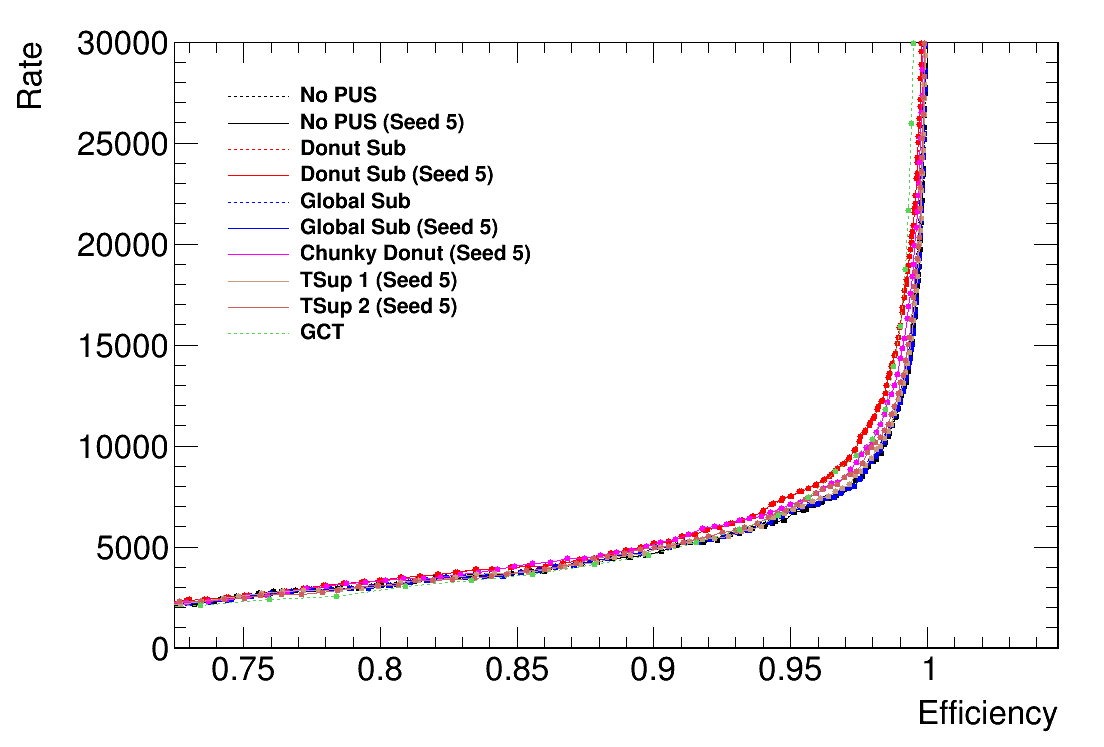
\includegraphics[width=0.5\textwidth]{./Figures/triggerUpgrade/singleJet_150.png}}~
    \subfigure[]{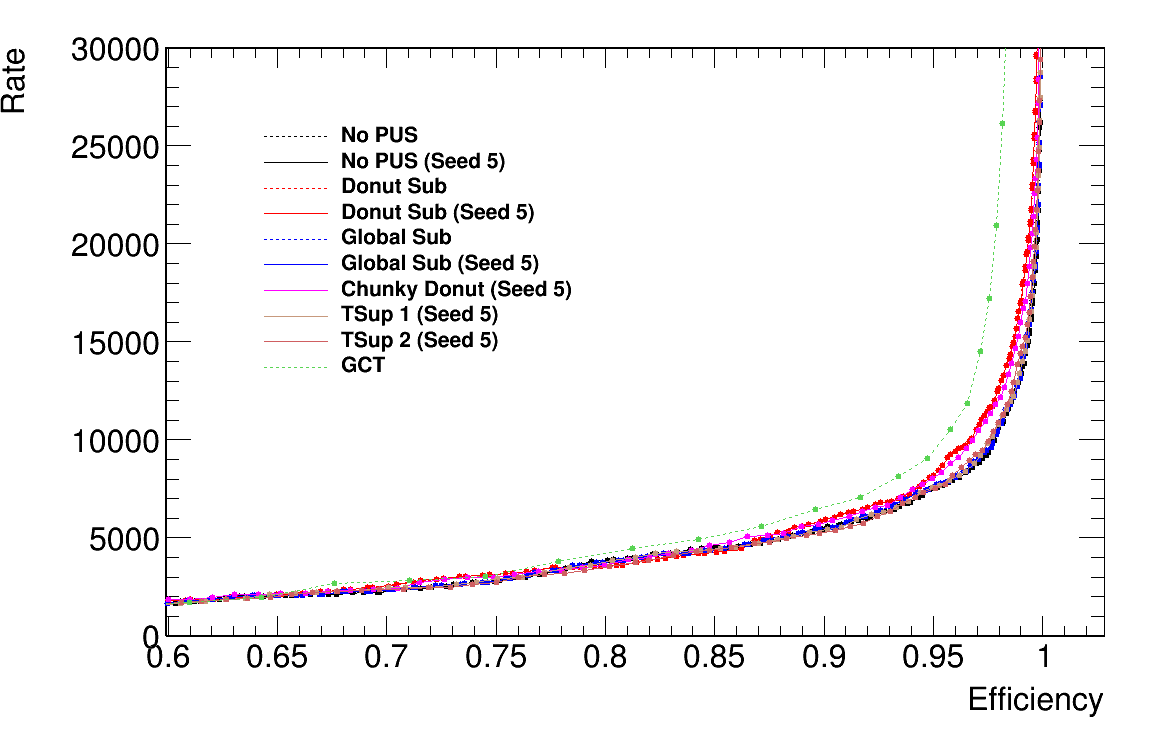
\includegraphics[width=0.5\textwidth]{./Figures/triggerUpgrade/doubleJet_110.png}}\\
    \subfigure[]{\includegraphics[width=0.5\textwidth]{./Figures/triggerUpgrade/quadJet_50.png}}
  \caption{\label{fig:rate_eff_jets} Rate against efficiency for (a) L1 leading jet with a threshold of 150\GeV, 
  (b) L1 second leading jet with a threshold of 110\GeV and (c) L1 fourth leading jet with a threshold of 50\GeV.}
\end{figure}

During Run 2 the pileup is not constant but varies with changes in instantaneous luminosity. 
Stability in the rate for different pileup scenarios is import to ensure that L1 trigger thresholds 
do not need to be increased during running. Figure~\ref{fig:rate_nvtx} shows the rate against the number of 
simultaneous interactions for a lead jet threshold of $30\GeV$. The dependence on pileup is 
seen to be significantly mitigated by chunky doughnut pileup subtraction compared to no pileup subtraction and global $\rho$
subtraction. 

\begin{figure}
\centering
    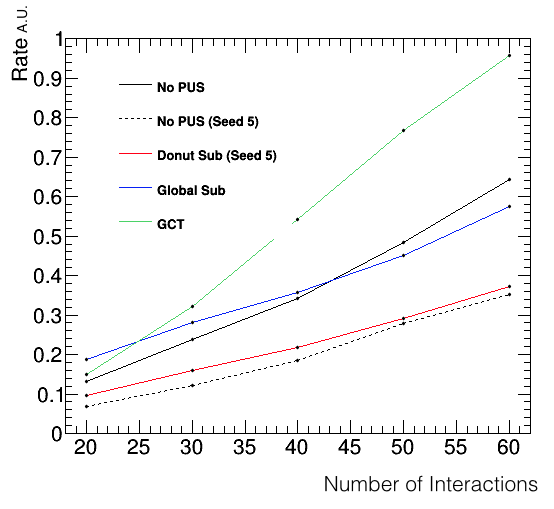
\includegraphics[width=0.8\textwidth]{./Figures/triggerUpgrade/neutrinonvtx_jet1}
  \caption{The dependence of the rate for a threshold of $\Lonept=30GeV$ on the number of simultaneous interactions}
  \label{fig:rate_nvtx}
\end{figure}

To benchmark the energy sums performance the rate against efficiency for L1 \scalht~and L1 \mht~is shown in Figure~\ref{fig:rate_eff_sum}.
All jets above $20\GeV$ are used to calculate L1 \scalht, making this quantity particularly susceptible to pileup. The chunky doughnut 
pileup subtraction with a seed of 5 is shown to significantly improve performance compared to the other pileup subtraction
methods and the legacy system\footnote{The performance of the UCT is not 
directly comparable as L1 \scalht~and \mht are calculated using calorimeter regions above a threshold
rather than jets} (except global $\rho$ with a seed of 5, not viable in the L1 trigger). Similarly, the performance for 
L1 \mht~is optimal for chunky doughnut subtraction with a seed of 5 and global $\rho$ subtraction. 
Figure~\ref{fig:mht_rateEff} also shows L1 $\met$~which exhibits the best performance. This is expected as 
pileup contributions are approximately uniformly deposited in $\phi$ throughout the detector and their contribution will
cancel in the vector sum of the towers.

\begin{figure}
\centering
	\subfigure[]{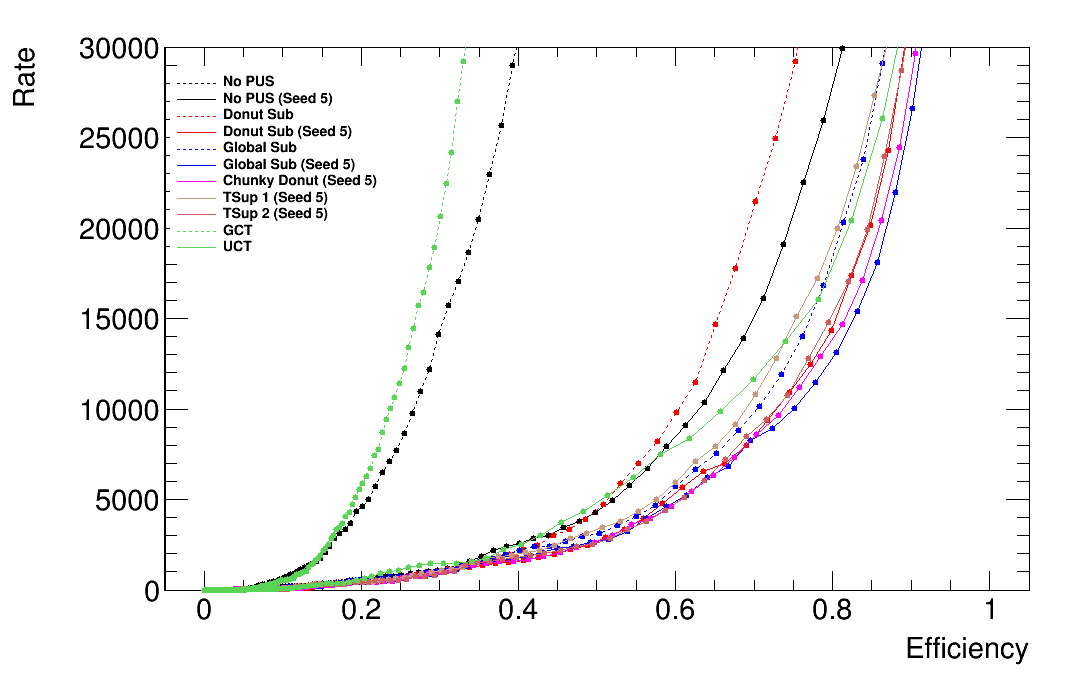
\includegraphics[width=0.5\textwidth]{./Figures/triggerUpgrade/ht_200}\label{fig:ht_rateEff}}~
	\subfigure[]{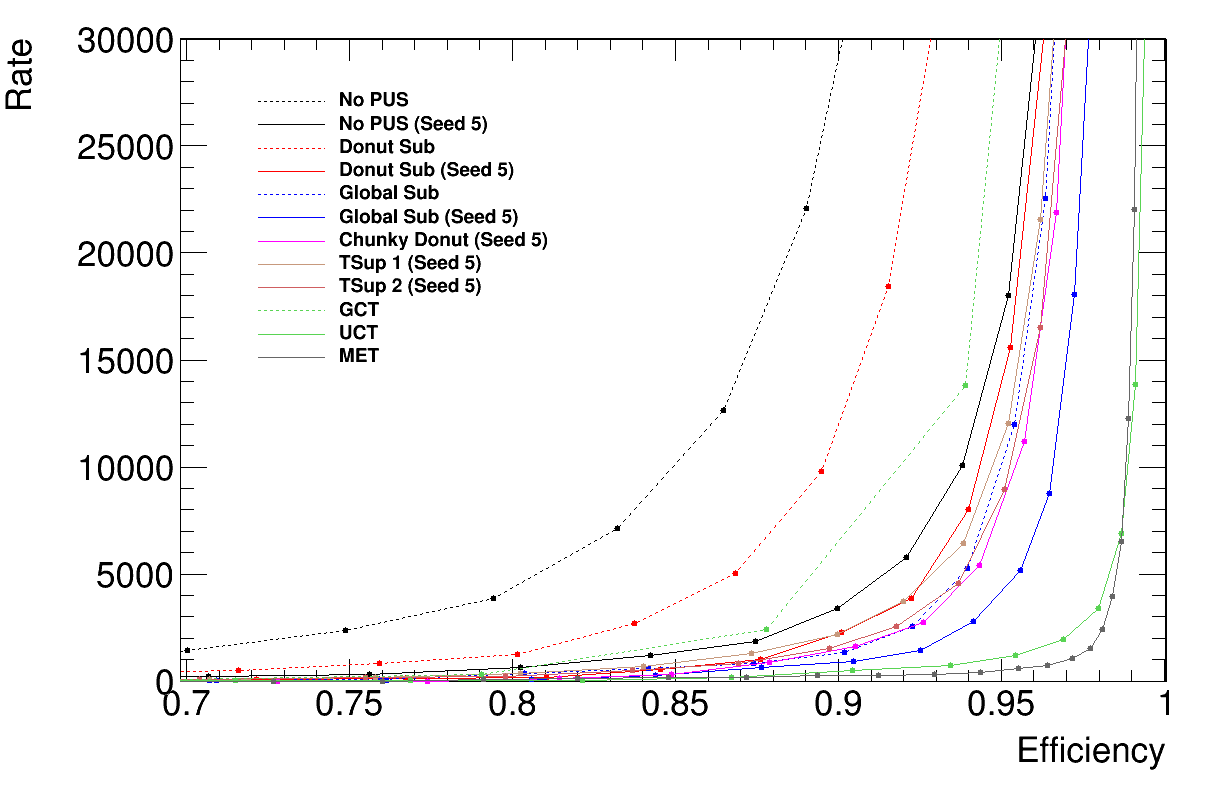
\includegraphics[width=0.5\textwidth]{./Figures/triggerUpgrade/mht_200}\label{fig:mht_rateEff}}
	\caption{Rate against efficiency for (a) L1 \scalht and (b) L1 \mht, both with a
	threshold of 200\GeV.}
	    \label{fig:rate_eff_sum}
\end{figure}

\subsection{Summary}

The performance plots described in this section have highlighted the importance of effective
pileup subtraction for the L1 trigger. Significantly improved performance is observed over 
the legacy and UCT systems, highlighting the advantages of additional granularity
and algorithmic complexity afforded by the upgraded architecture.
The best performance is seen with the chunky doughnut (with a seed threshold) 
and global~$\rho$ pileup subtraction. Due to latency constraints and the desire to account for 
local effects when triggering, a local pileup subtraction algorithm is preferred. 
Therefore, the chunky doughnut subtraction has been used for data taking in 2016.

Figure~\ref{fig:trig_2016} shows two example performance plots made using early 2016 data. 
The upgrade jet energy is seen to agree well with offline over a wide range of energies 
and shows little pileup dependence.


\begin{figure}
\centering
	\subfigure[]{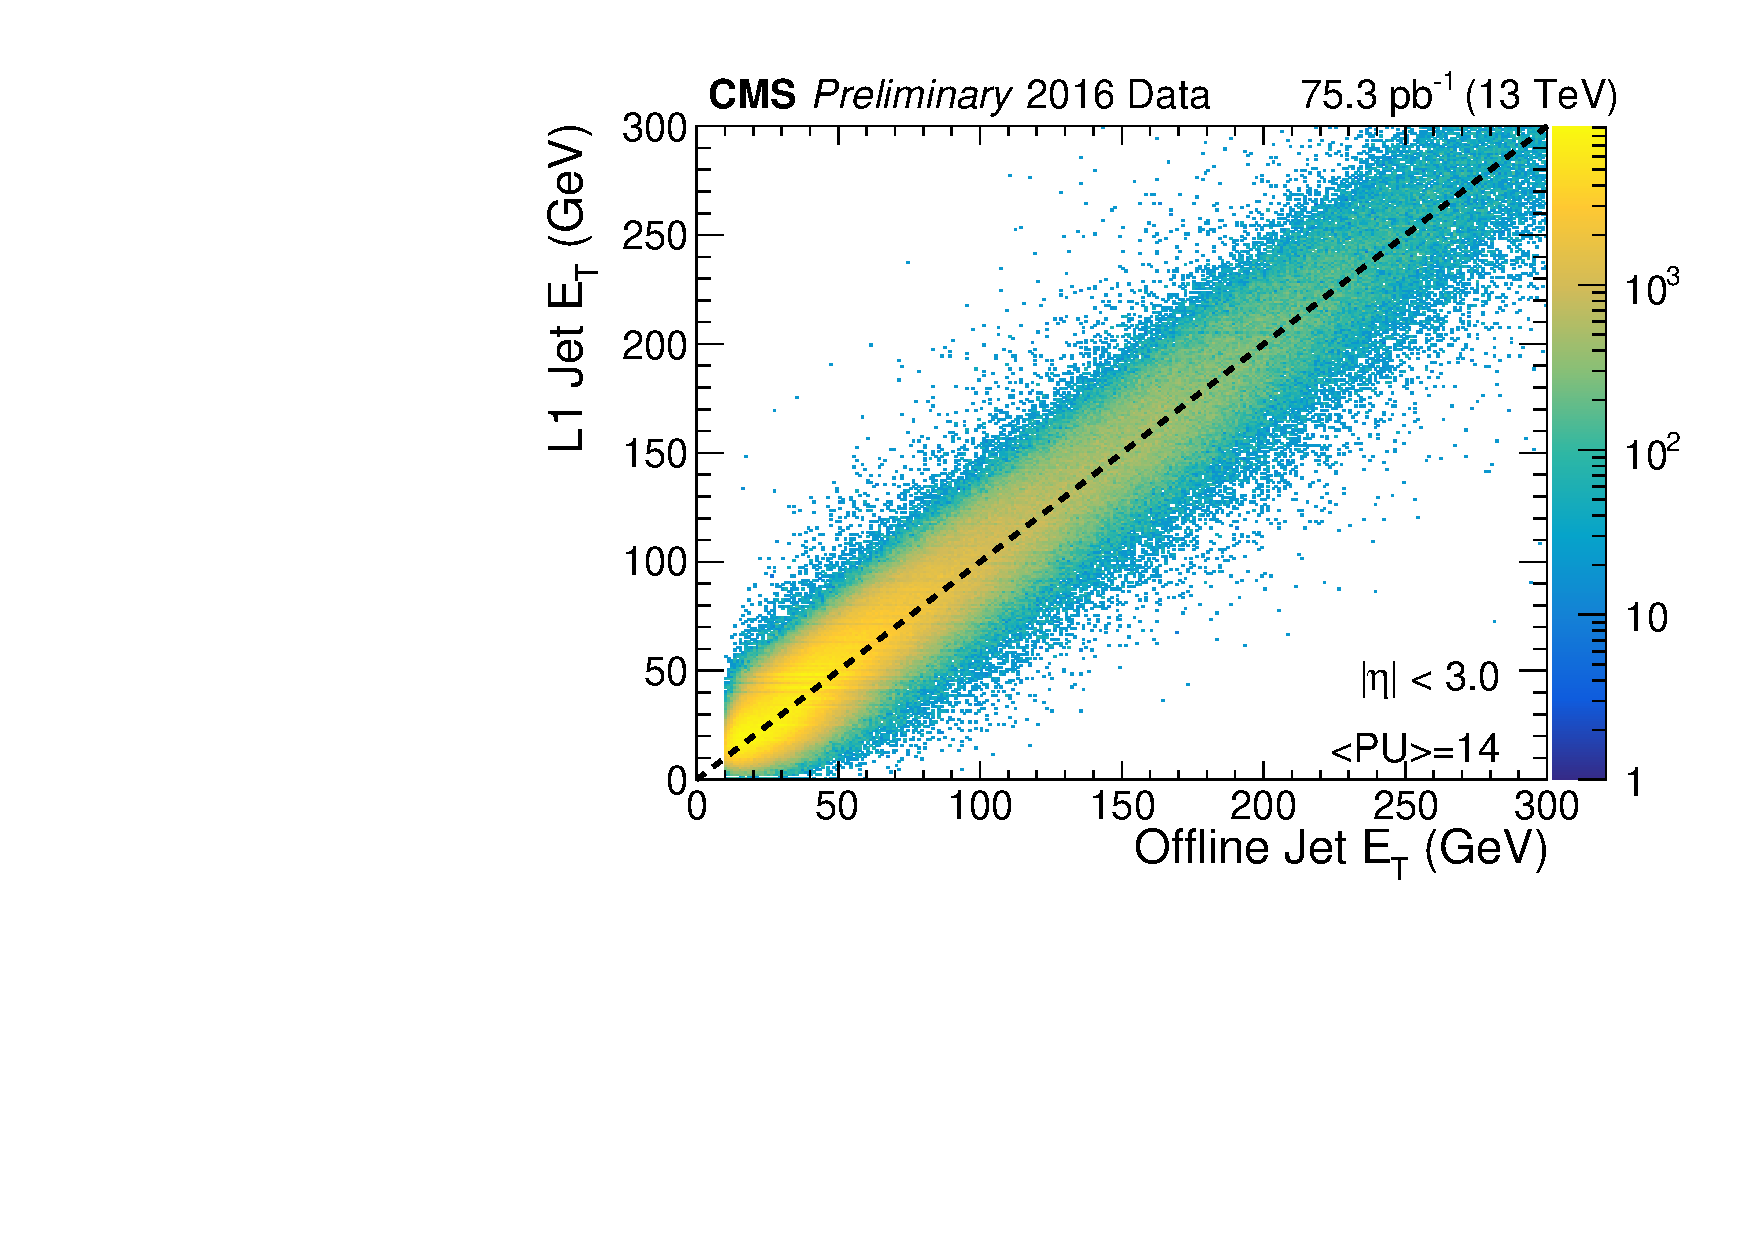
\includegraphics[width=0.5\textwidth]{./Figures/triggerUpgrade/xy_SingleMu_jetEt_vs_l1JetEt_barrel-endcap}}~
	\subfigure[]{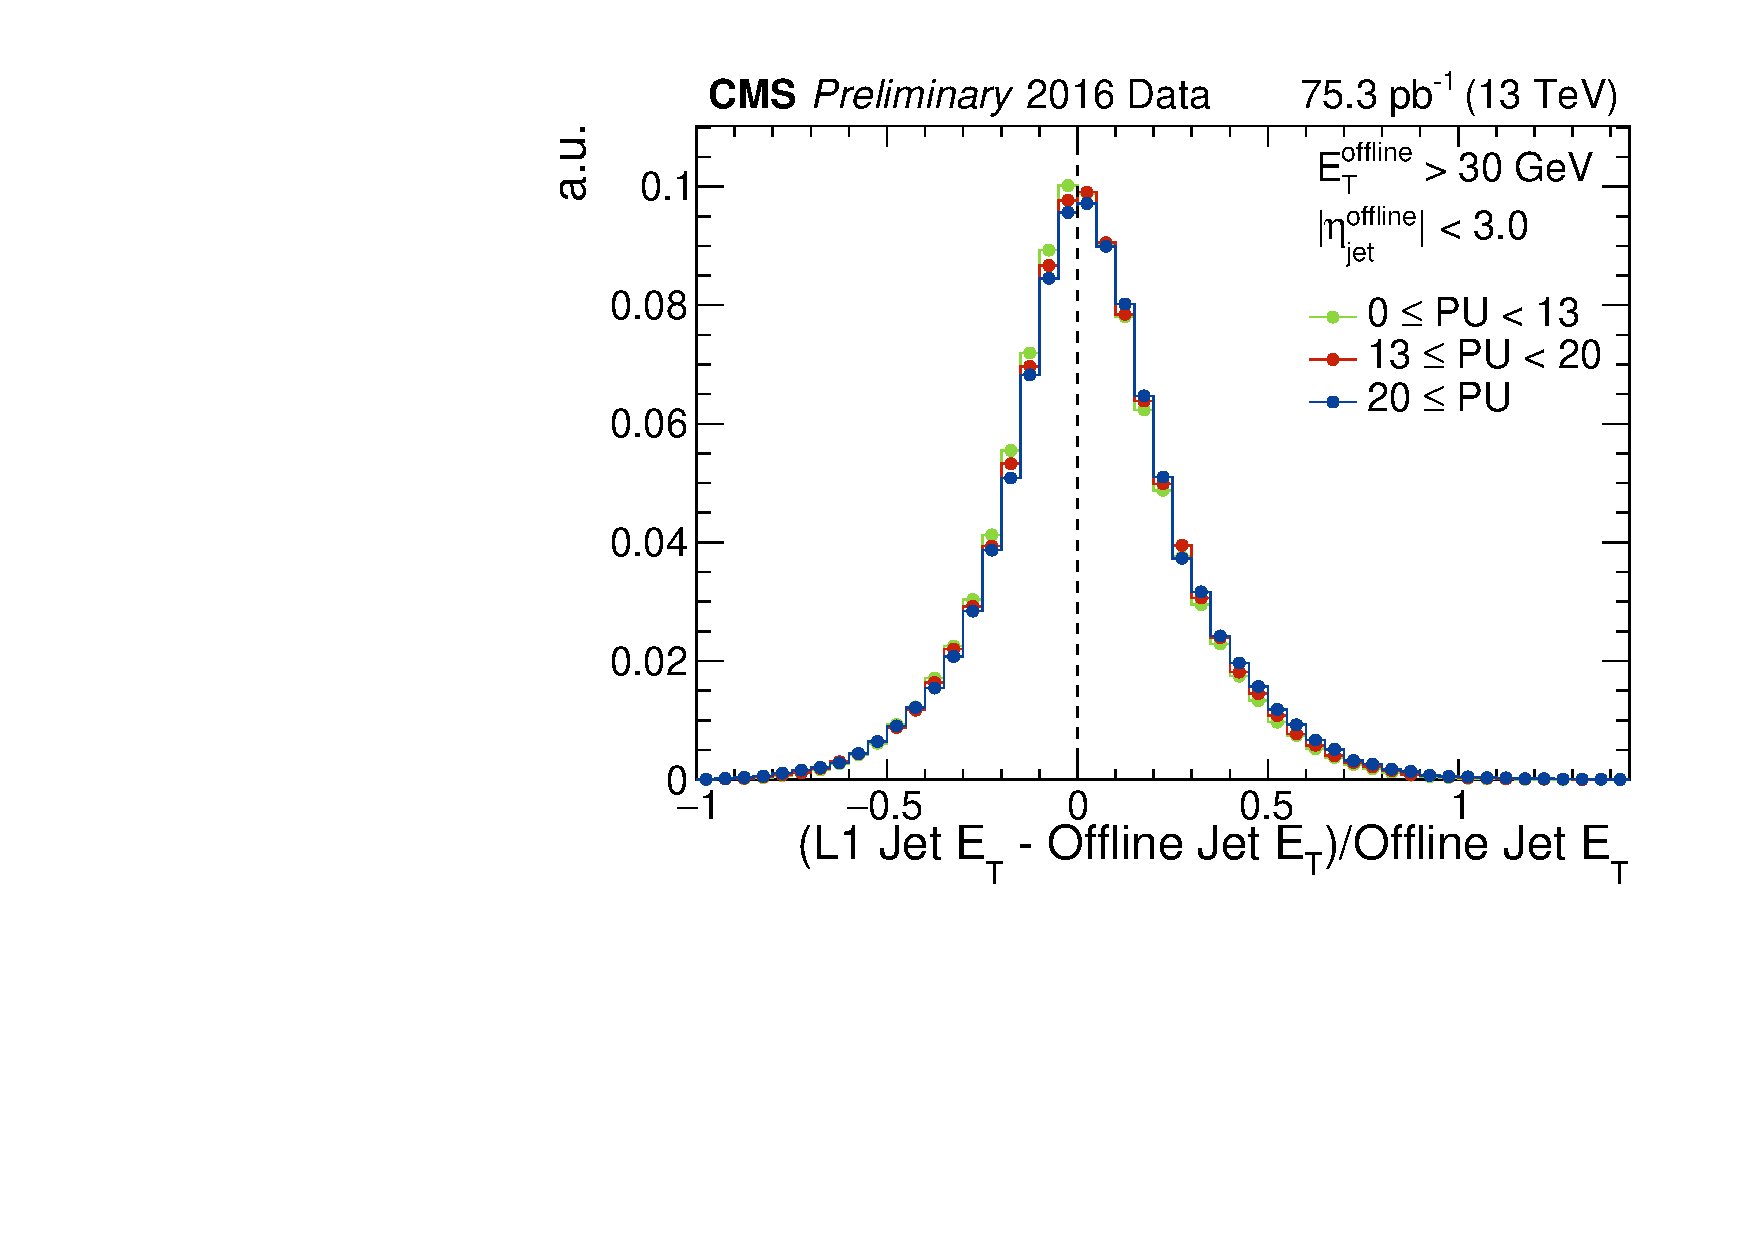
\includegraphics[width=0.5\textwidth]{./Figures/triggerUpgrade/res_SingleMu_jetEt_over_l1JetEt_barrel-endcap_puBins}}
	\caption{(a) The L1 jet energy compared to offline in early 2016 data for a wide
range of jet energies. (b) Resolution for the L1 jet energy compared to offline in early 2016 data for several different 
pileup scenarios \cite{l1sums_perf}.}
\label{fig:trig_2016}
\end{figure}


\section{Cross trigger study}
\label{sec:cross_trigger}
The simple single object triggers considered in the previous section are useful for selecting
high \pt~signatures and for low luminosities. In order to provide efficiency for
the full range of the CMS physics program at higher luminosities, sophisticated combinations
of the single object triggers, \emph{cross triggers}, are required. In this section, the \alphat 
analysis is used to highlight the utility of such a cross trigger at L1. 

The \alphat analysis is fully described in Section ??. In order to maximise the acceptance
to supersymmetric models at lower energy scales a low \scalht~threshold is required. 
However, without an additional requirement, the rate
would be unacceptably high. A cross trigger using a combined selection on the difference 
in $\phi$ between the two leading jets ($\Delta\phi_{1,2}$) and \scalht can control this rate while 
maintaining efficiency. The $\Delta\phi_{1,2}$ requirement takes advantage of the high relative 
\mht to \scalht for the signal models.

An acceptable rate for such a cross trigger, given the overall budget of 100kHz, is 
around 5.5 to 7.5 kHz. This range defines a band in the plane of $\Delta\phi_{1,2}$
and \scalht~in which the efficiency can be inspected. To avoid signal model dependence, the 
efficiency is measured using a \ttbar sample for the multijet case ($\nj \ge 4$) and a sample  
of Z boson production in association with jets, where the Z decays to neutrinos, for the 
dijet case ($\nj == 2$). An offline hadronic selection of $200 < \scalht < 300$ 
and $\alphat > 0.65$ is made in defining the efficiency. This approximates to the selection
of the lowest \scalht~regions used in the \alphat~search, for which achieving high efficiencies is most challenging.
The results are shown for both the TMT and UCT trigger in Figures~\ref{fig:dijet_cross} and~\ref{fig:multijet_cross} 
for the dijet and multijet trigger respectively. For the TMT, chunky doughnut corrected, calibrated jets are used.

\begin{figure}
\centering
	\subfigure[Upgrade trigger]{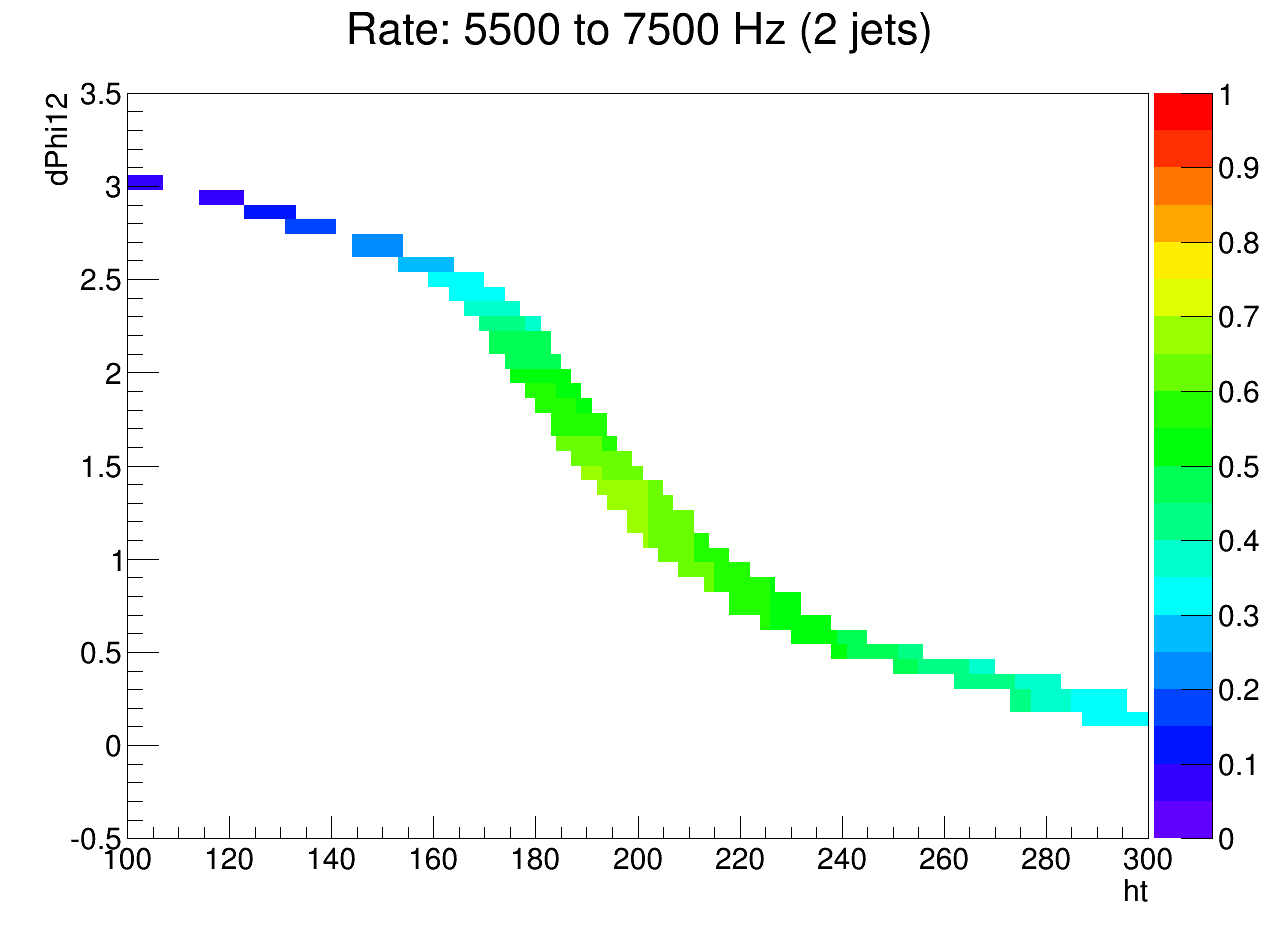
\includegraphics[width=0.5\textwidth]{./Figures/triggerUpgrade/noHardBin12JetdphiFullS2}}~
	\subfigure[UCT]{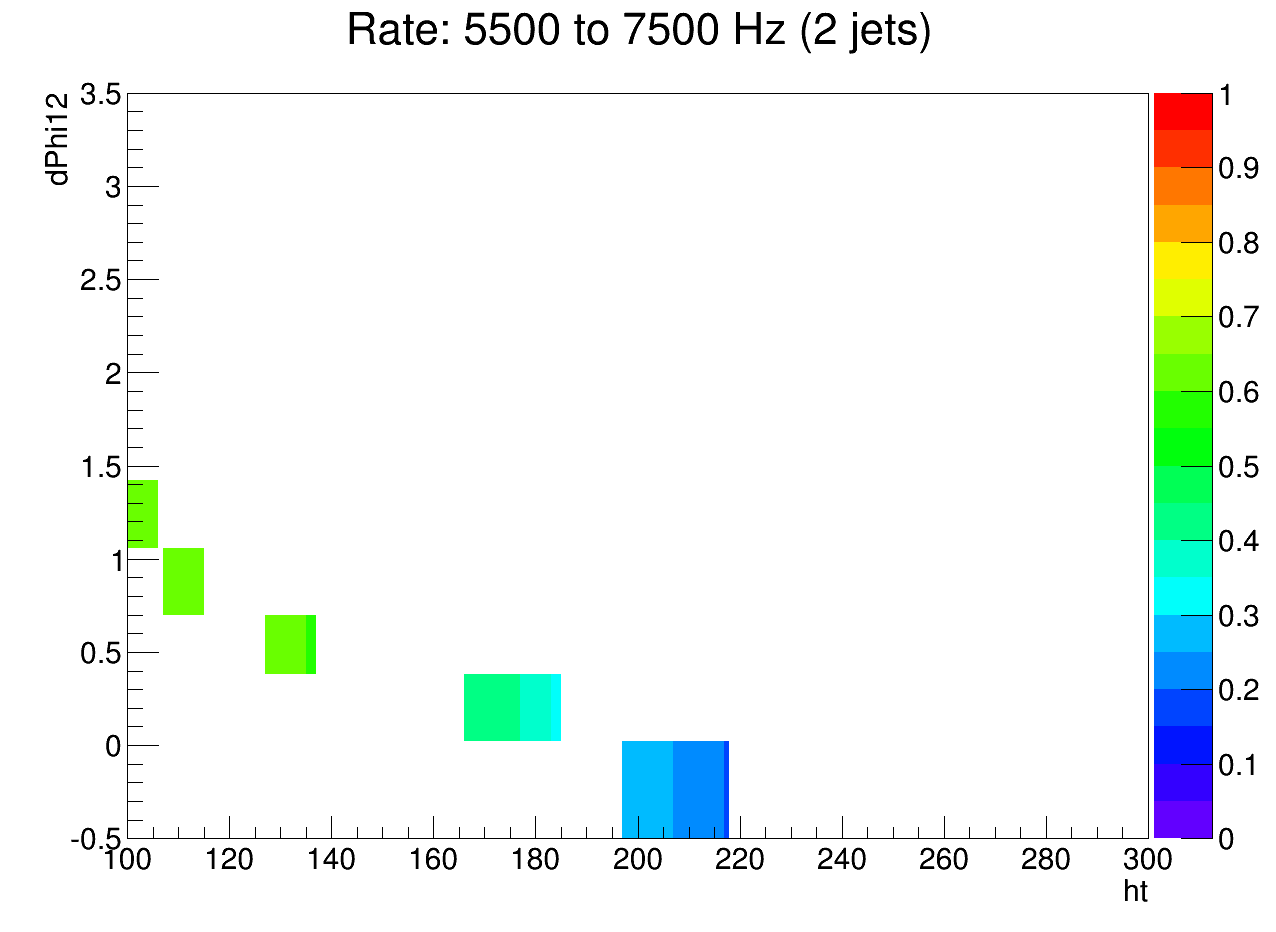
\includegraphics[width=0.5\textwidth]{./Figures/triggerUpgrade/noHardBin12JetdphiFullUCT}}
	\caption{Efficiency of the dijet selection for hadronic offline requirement $200 < \scalht < 300$ and $\alphat > 0.65$
	in a band of rate of 5.5 to 7.5 kHz}
	    \label{fig:dijet_cross}
\end{figure}

\begin{figure}
\centering
	\subfigure[Upgrade trigger]{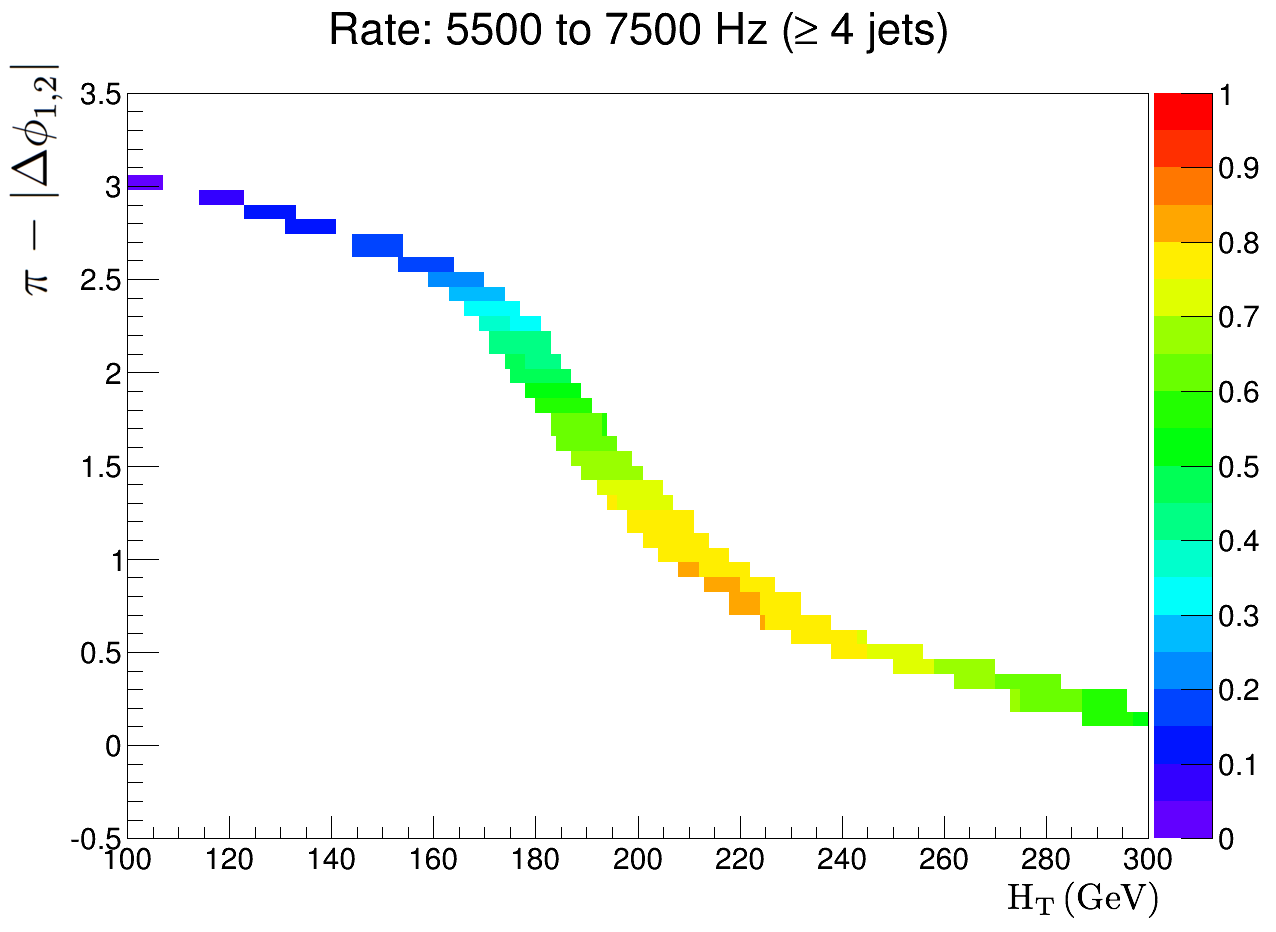
\includegraphics[width=0.5\textwidth]{./Figures/triggerUpgrade/noHardBin1ge4JetdphiFullS2}}~
	\subfigure[UCT]{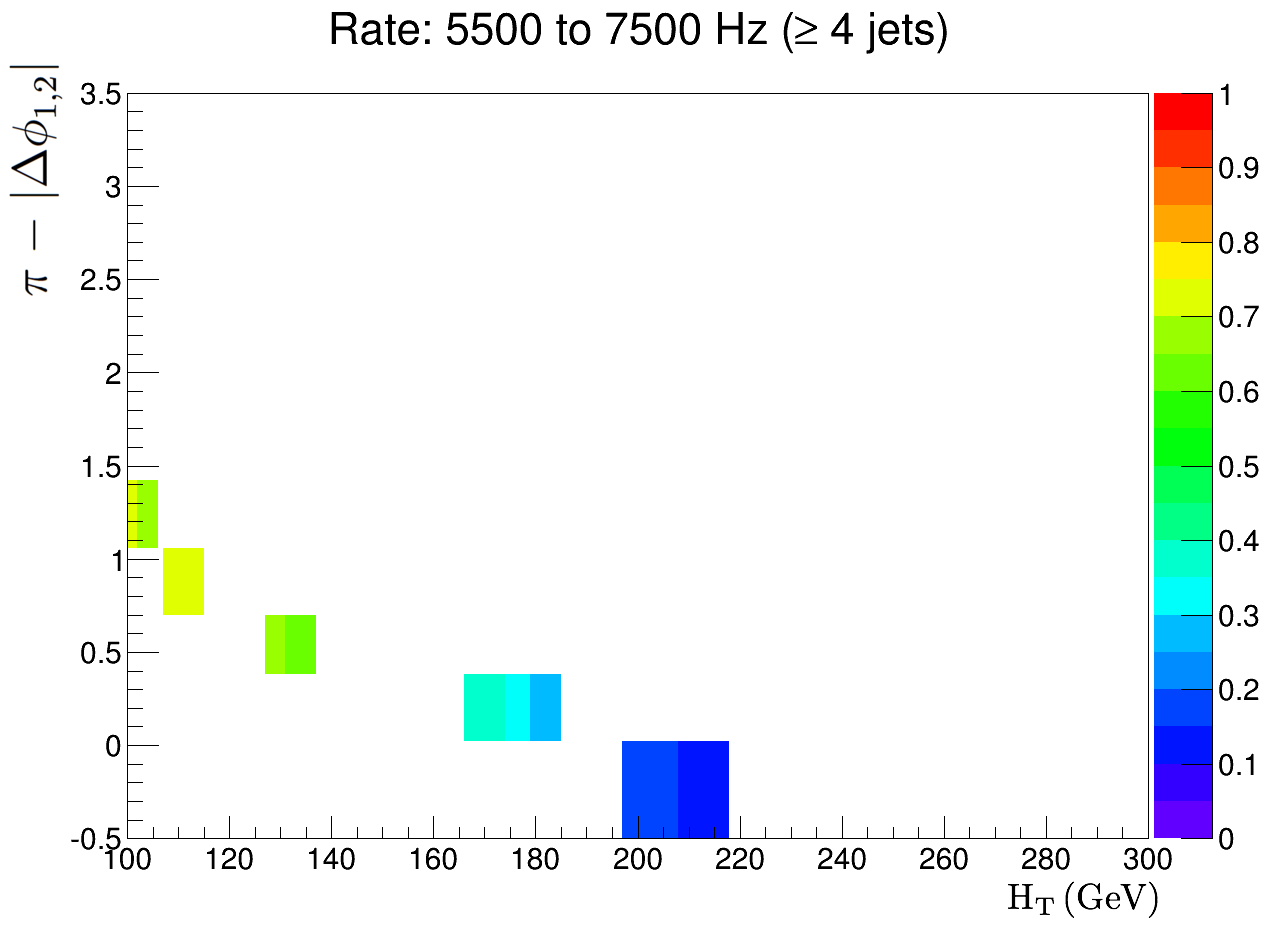
\includegraphics[width=0.5\textwidth]{./Figures/triggerUpgrade/noHardBin1ge4JetdphiFullUCT}}
	\caption{Efficiency of the multijet selection for hadronic offline requirement $200 < \scalht < 300$ and $\alphat > 0.65$
	in a band of rate of 5.5 to 7.5 kHz}	
	    \label{fig:multijet_cross}
\end{figure}

In both cases the greatly superior resolution afforded by the TMT allows a significantly
more granular operating range than the UCT. Addtionally, Higher efficiencies, especially for the multijet topology, 
are achievable for the upgraded system. The maximal efficiency gain in using $\Delta\phi_{1,2}$ to 
to that using a \scalht~trigger alone may also be considered for the TMT. For the dijet case there is a 
significant efficiency gain from $\sim 30\%$ to $\sim 70\%$, while for the multijet the gain is 
$\sim 50\%$ to $\sim 80\%$ when $\Delta\phi_{1,2}$ is used in conjunction with \scalht.
This highlights the importance of cross triggers in controlling rates while 
keeping low offline thresholds.

